\documentclass{astroedu-lab}

\begin{document}

\pagestyle{plain}

\begin{problem}{\huge Радиотехническая работа 24\\\\Безынерционные линейные цепи\\\\Выполнил Жданов Елисей Б01-205}

\section{Оборудование:}

Программное обеспечание MicroCap 10.0.7.0

\section{\textbf{model 1 (Тепловой шум Джонсона)}}

\subsection*{\textbf{model 1\_1 (Первое знакомство)}}

\begin{enumerate}

\item

Исследуем модель резистора как источника шумового напряжения, изучим зависимость шумового напряжения от R, получим что шум растет как $\sqrt{R}$.

\begin{figure}[h!]
    \centering
    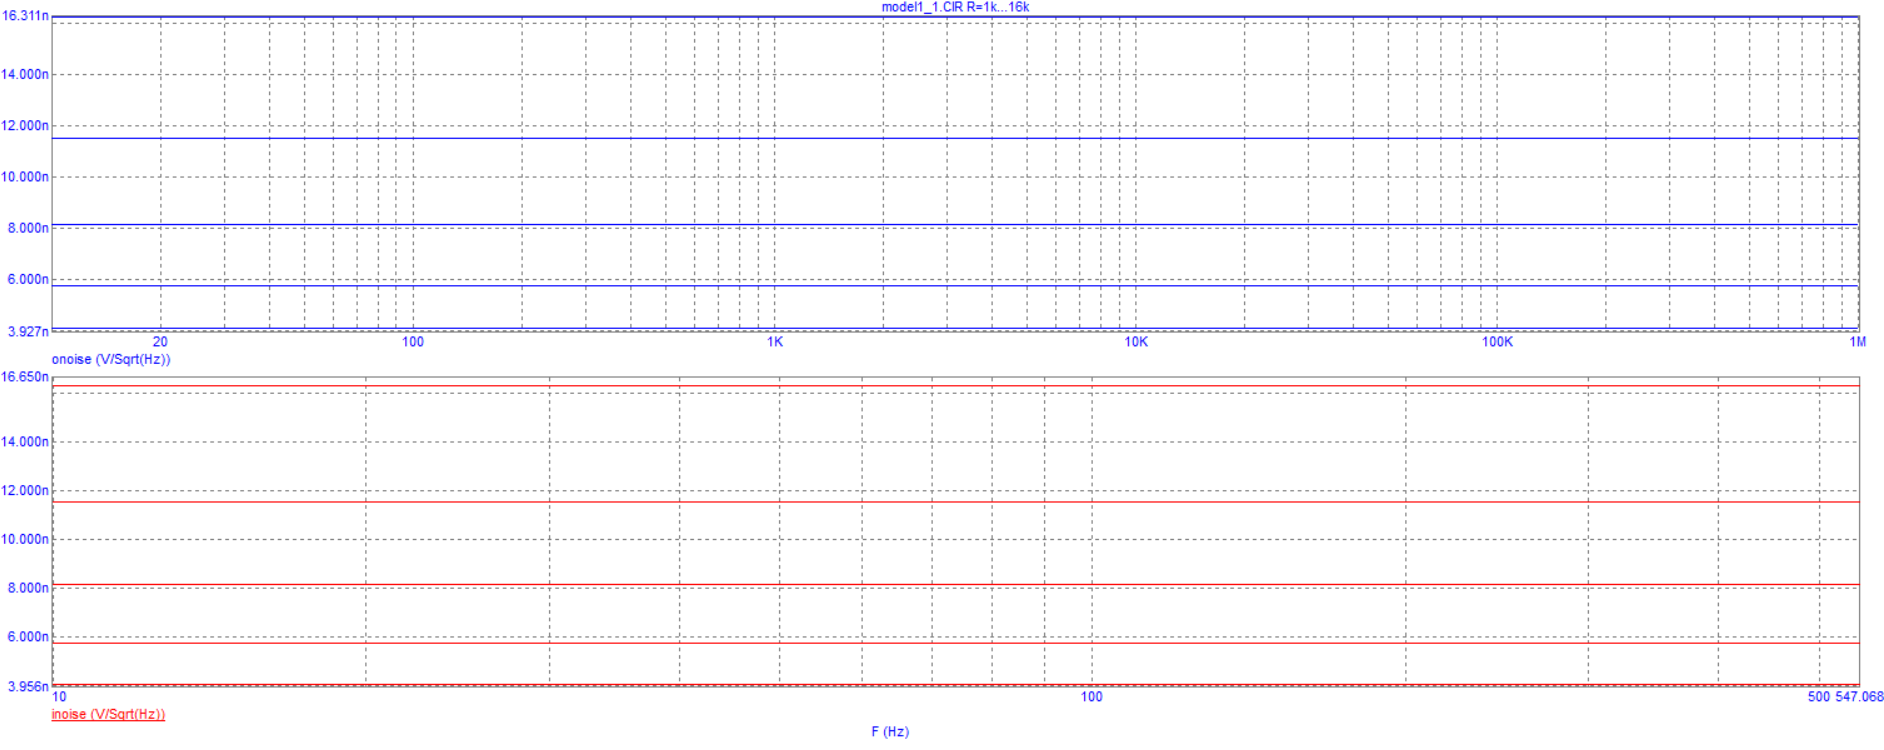
\includegraphics[scale=0.3]{images/mod1_1_1_2.png}
    \caption{Зависимость шумового напряжения от R}
    \label{fig:eR}
\end{figure}

\item

Измерим уровень шума $\sigma$ на выводе резистора в полосе F = 1 МГц.

\begin{figure}[h!]
    \centering
    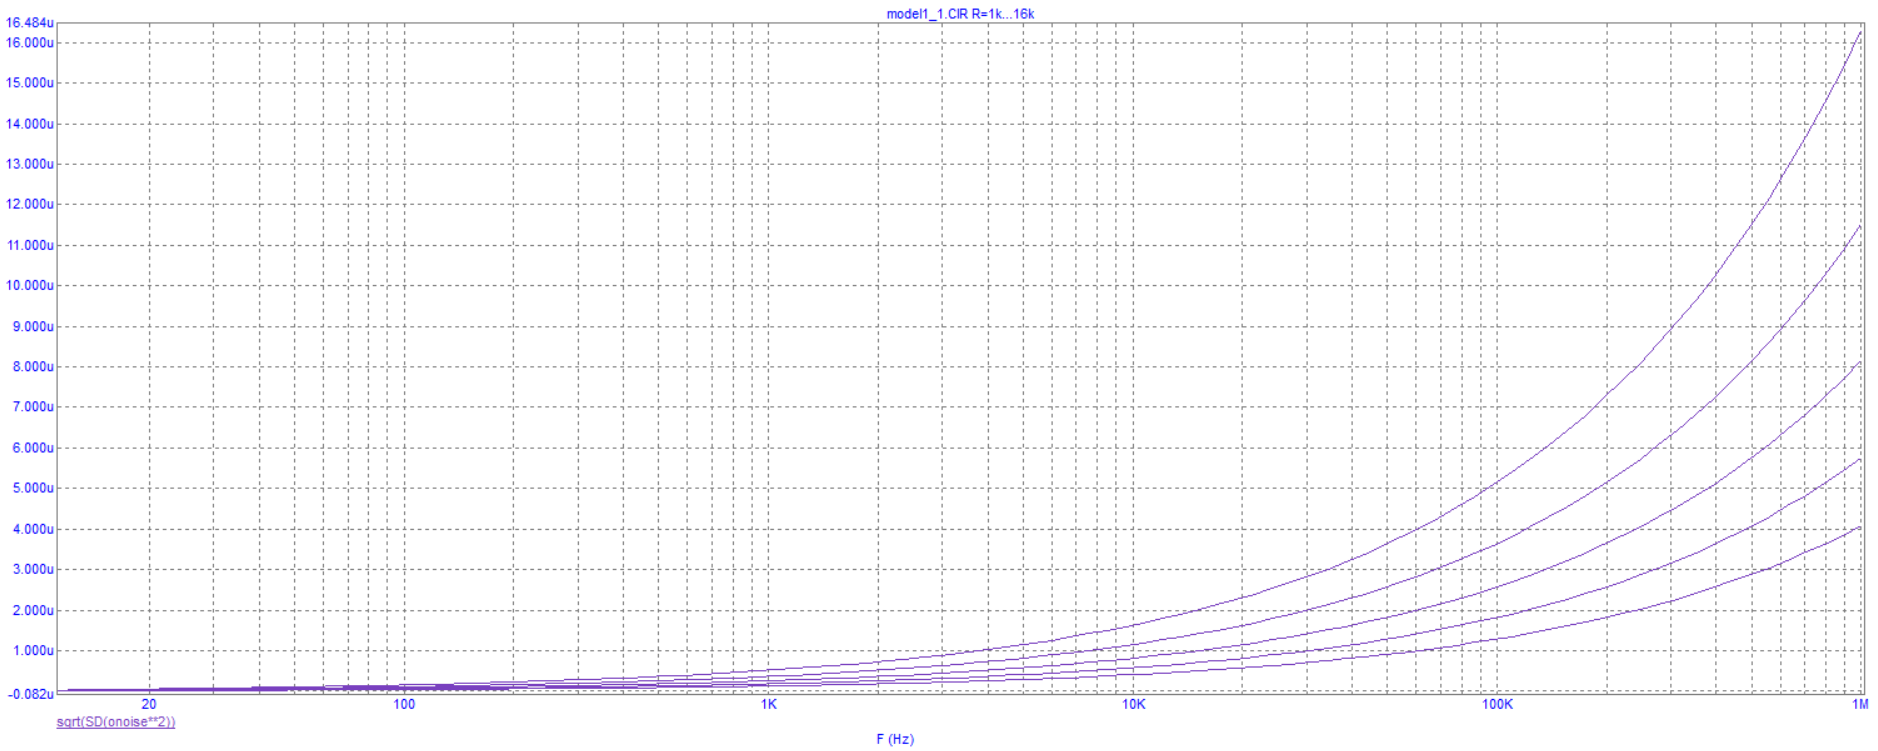
\includegraphics[scale=0.3]{images/mod1_1_2_1.png}
    \caption{R = [1k, 16k| Log2]}
    \label{fig:R16}
\end{figure}

\begin{figure}[h!]
    \centering
    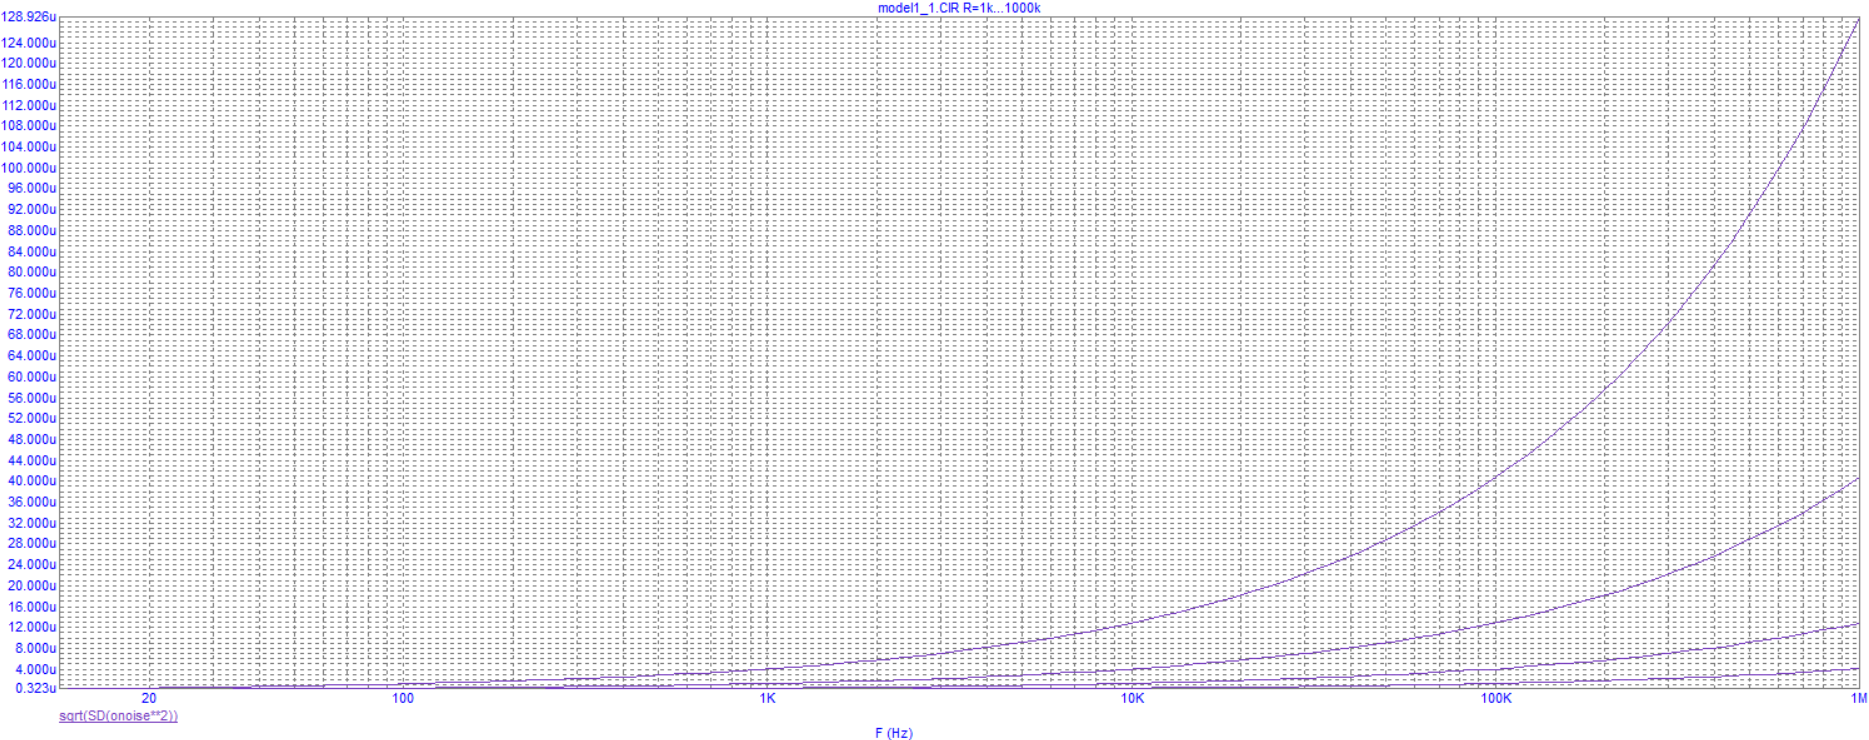
\includegraphics[scale=0.3]{images/mod1_1_2_2.png}
    \caption{R = [1k, 1000k| Log10]}
    \label{fig:R1000}
\end{figure}

\begin{center}
\begin{table}[h!]
    \centering
    \begin{tabular}{|c|c|c|c|c|c|c|c|c|} \hline
        R & 1k & 2k & 4k & 8k & 16k & 10k & 100k & 1000k\\ \hline
        $\sigma$ & 4u & 5,7u & 8u & 11,4u & 16u & 12,7u & 40u & 128u\\ \hline
    \end{tabular}
    \caption{Зависимость уровня шума $\sigma$ от R}
    \label{tab:sR}
\end{table}
\end{center}

\item

Перейдем к модели источника тока, получаем, что с увеличением R1 ток падает как $1/\sqrt{R}$(необходимо увеличить масштаб), а напряжение растет как $\sqrt{R}$.

\begin{figure}[h!]
    \centering
    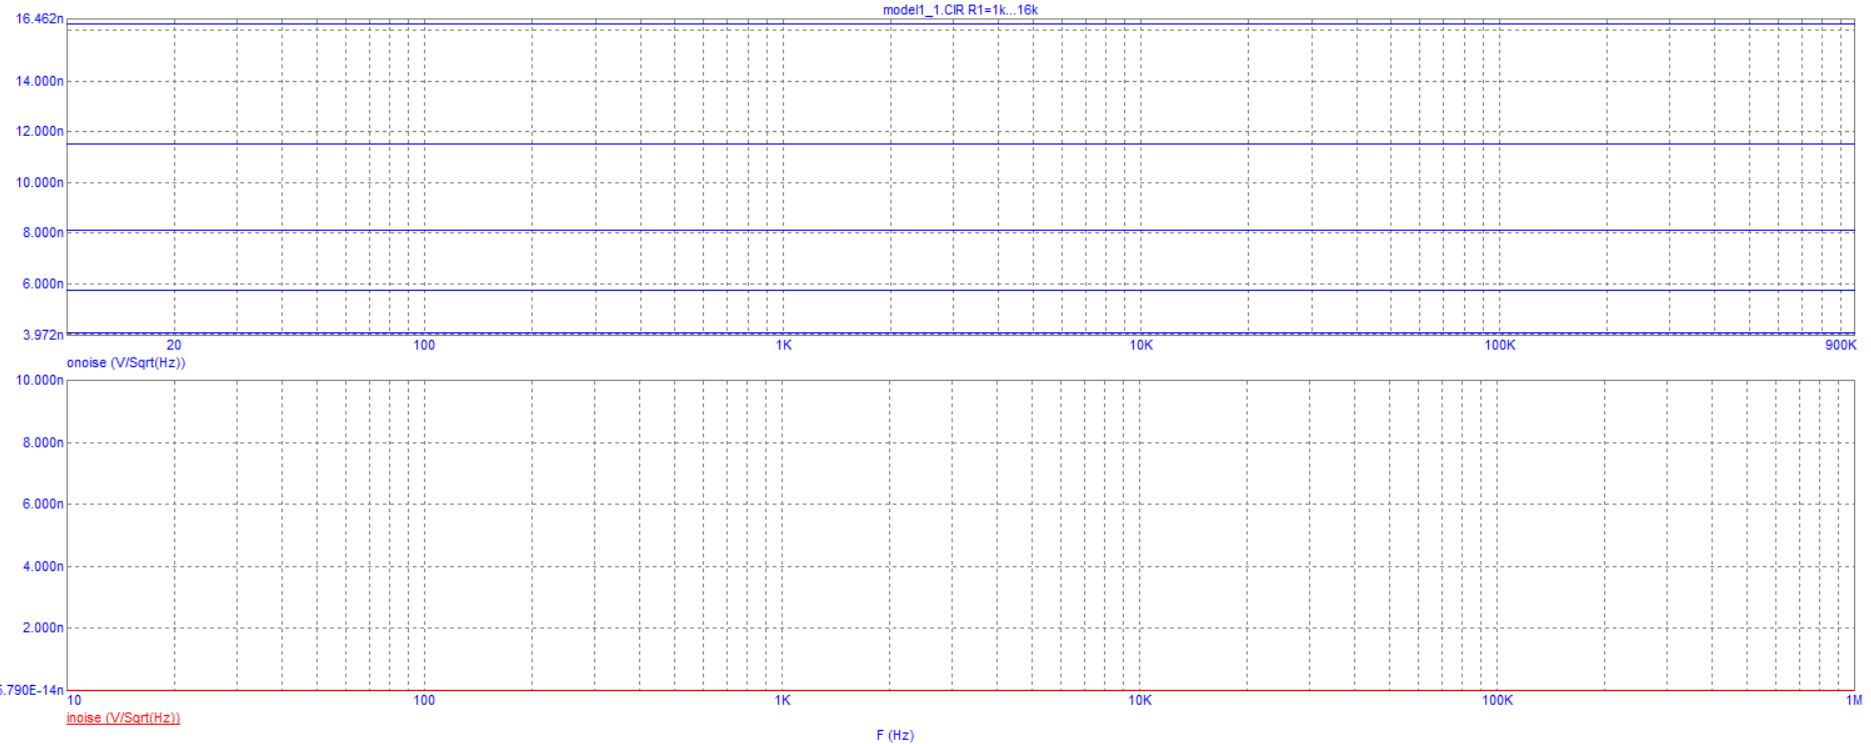
\includegraphics[scale=0.3]{images/mod1_1_3.png}
    \caption{Шумовые напряжение и ток в модели с источником тока}
    \label{fig:R3}
\end{figure}

\end{enumerate}

\subsection*{\textbf{model 1\_2 (Сложение шумов)}}

\begin{enumerate}

\item

Изучим шумы в схеме с последовательным соединением, проверим закон сложения шумовых напряжений.

\begin{figure}[h!]
    \centering
    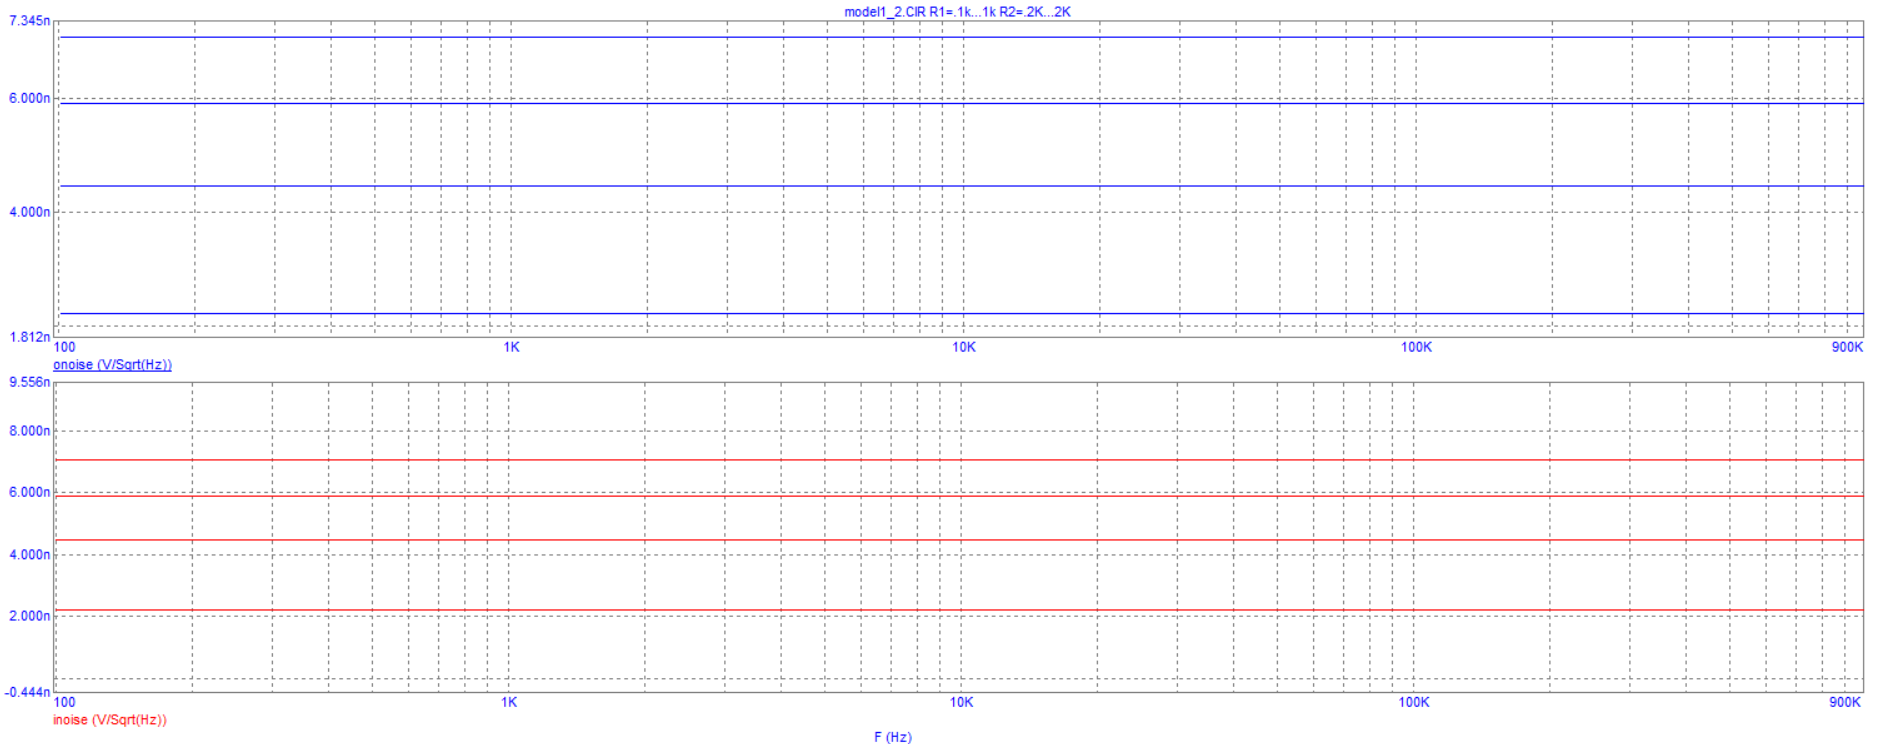
\includegraphics[scale=0.3]{images/mod1_2_1.png}
    \caption{Варьирование R = [0,1k, 1k| 1k], R = [0,2k, 2k| 2k]}
    \label{fig:1_2_1}
\end{figure}

Закон сложения шумовых напряжений выполняется.

\item
 
Перейдем к схеме с параллельным соединением (рис. 6). Закон сложения шумовых токов выполняется.

\begin{figure}[h!]
    \centering
    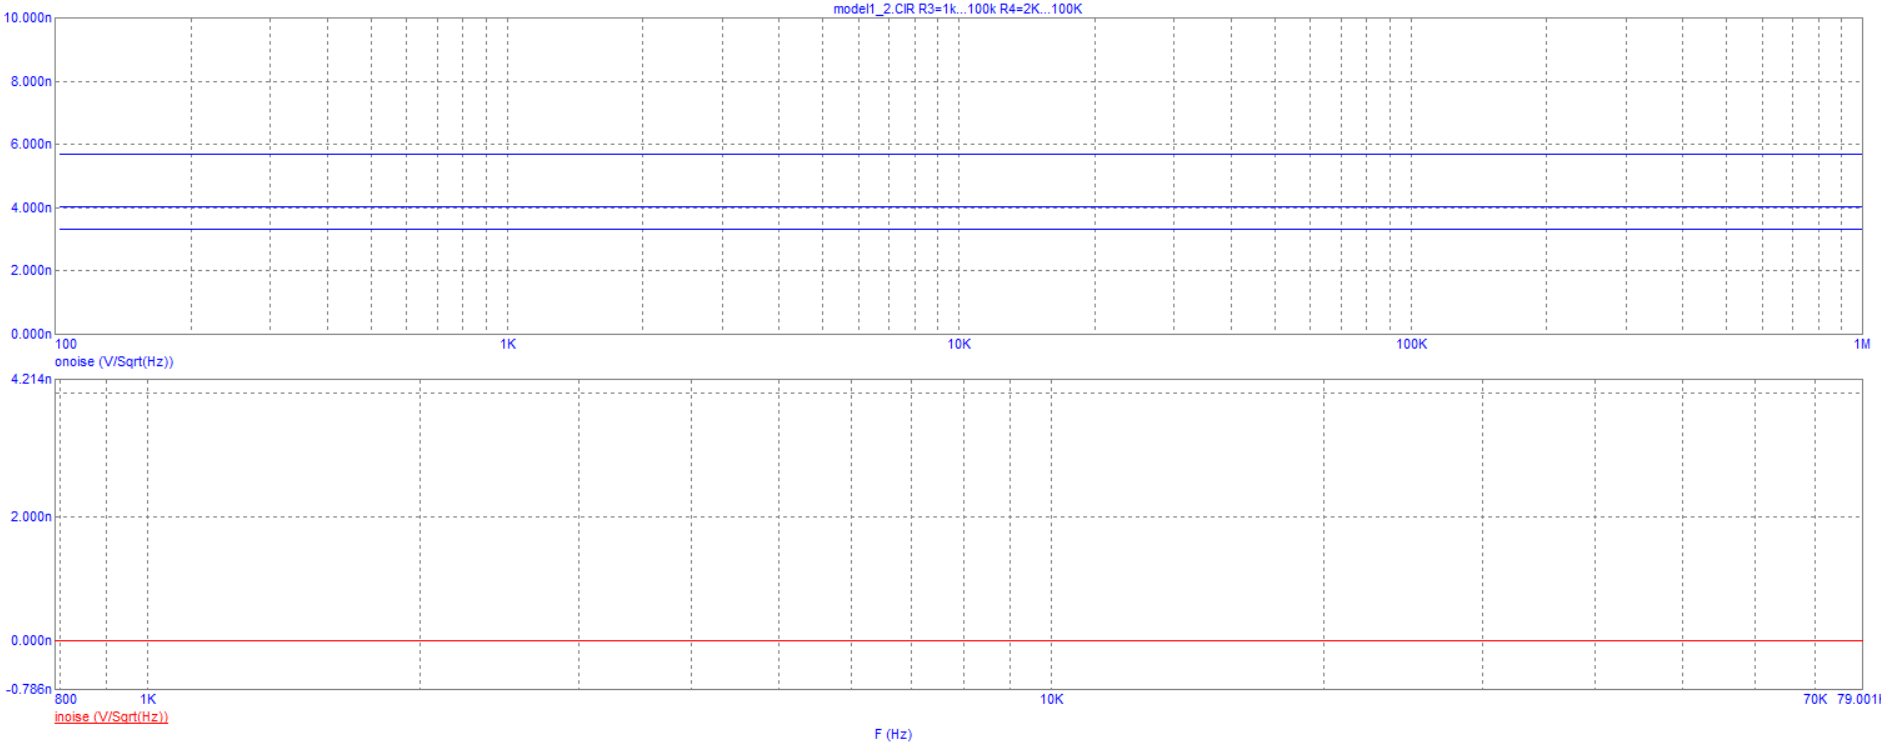
\includegraphics[scale=0.3]{images/mod1_2_2.png}
    \caption{Варьирование R = [1k, 100k| 99k], R = [2k, 100k| 98k]}
    \label{fig:1_2_2}
\end{figure}

\end{enumerate}

\subsection*{\textbf{model 1\_3 (Шум в делителе напряжения)}}

\begin{enumerate}

\item

Измерим шумовое напряжение в узле $n(f) = 5,2 \text{ нB}\sqrt{\text{Гц}}$. 

\pgfplotstableread[col sep = semicolon]{KT.csv}{\tabl}

\begin{figure}[h!]
    \centering
    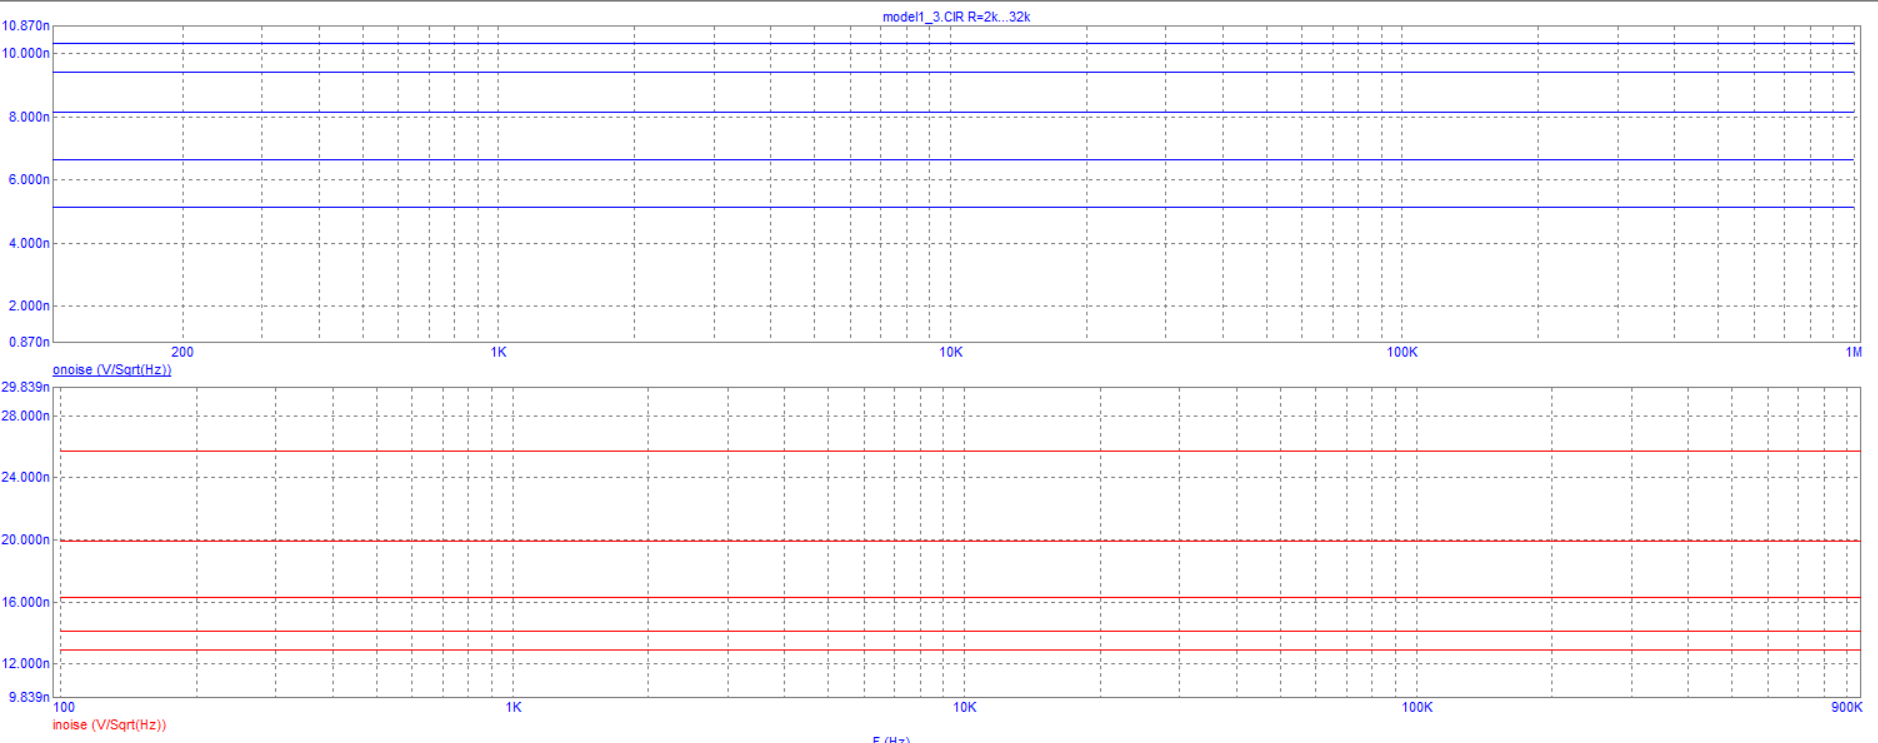
\includegraphics[scale=0.3]{images/mod1_3_1.png}
    \caption{Приведенное ко входу напряжение $e_n$ от R}
    \label{fig:1_3_1}
\end{figure}

\begin{tikzpicture}
\begin{axis}[title = $K_n(R)$,]
\addplot table [x={R}, y={K}] {\tabl};
\end{axis}
\centering
\end{tikzpicture}

\begin{tikzpicture}
\centering
\begin{axis} [title = $T_n(R)$]
\addplot table [x={R}, y={T}] {\tabl};
\end{axis}
\end{tikzpicture}

\item 

Исключим резистор R и поставим вместо него нешумящий резистор H. 

\begin{figure}[h!]
    \centering
    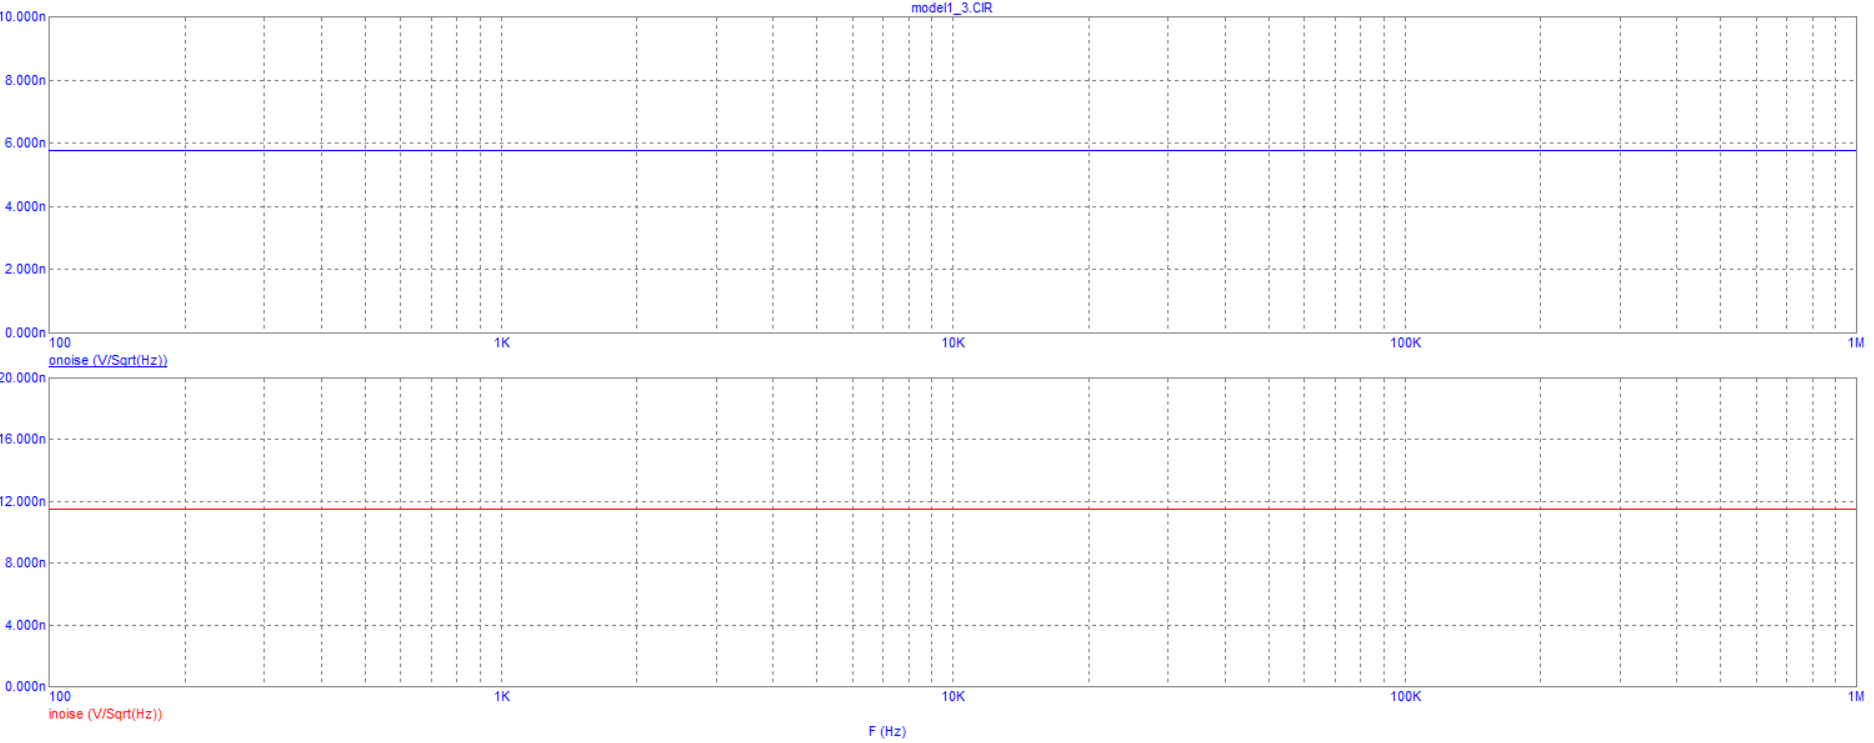
\includegraphics[scale=0.3]{images/mod1_3_2.png}
    \caption{Нешумящий резистор}
\end{figure}

При подстановке в формулы $R_s = 8$ кОм и $e_n = 11.515 $ нВ, действительно получим $K_n == T_n == 0$.

\end{enumerate}

\section{\textbf{model 2 (Дробовой шум диода Шоттки)}}

\newpage

\begin{enumerate}

\item

Проверим выполнение закона $\sqrt{I_0}$:
\begin{itemize}
    \item $I_{01} = 1\mu$ => $e_{01} = 566f$;
    \item $I_{02} = 10\mu$ => $e_{02} = 1.79p \approx \sqrt{10}e_{01}$;
    \item $I_{03} = 100\mu$ => $e_{03} = 5.659p \approx \sqrt{100}e_{01}$; 
    \item $I_{04} = 1000\mu$ => $e_{04} = 17.832p \approx \sqrt{1000}e_{01}$;
\end{itemize}

\begin{figure}[h!]
    \centering
    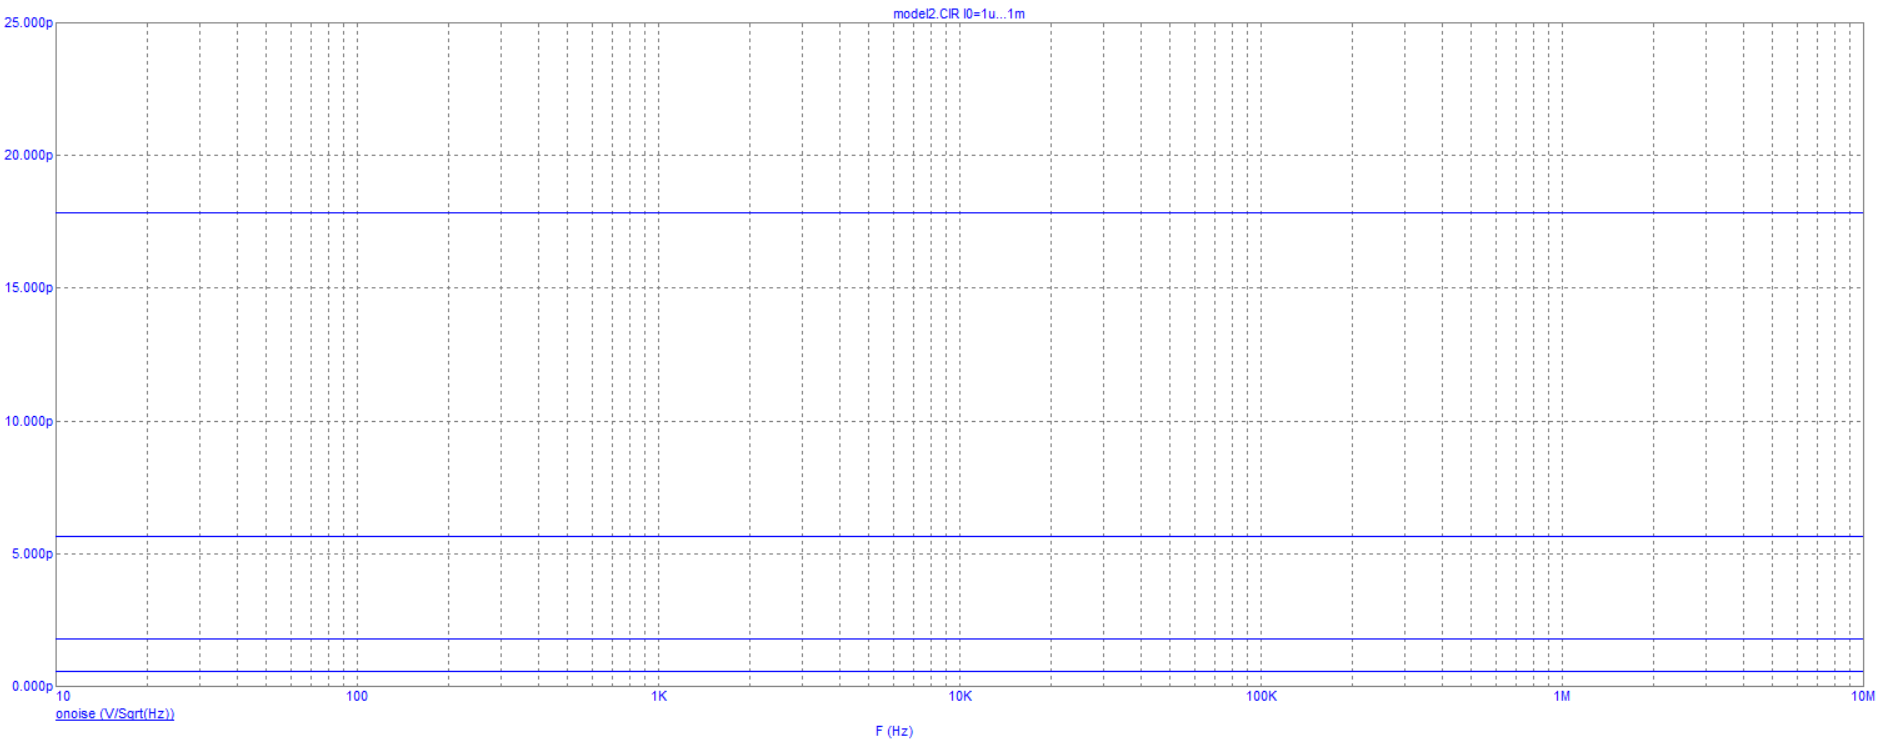
\includegraphics[scale=0.3]{images/mod2_1_1.png}
    \caption{Микротоки(2 1 1)}
    \label{fig:m211}
\end{figure}

Проверим выполнение закона $\sqrt{I_0}$:
\begin{itemize}
    \item $I_{01} = 1\mu$ => $e_{01} = 17.83p$;
    \item $I_{02} = 2\mu$ => $e_{02} = 25.12p \approx \sqrt{2}e_{01}$;
    \item $I_{03} = 4\mu$ => $e_{03} = 35.26p \approx \sqrt{4}e_{01}$; 
    \item $I_{04} = 8\mu$ => $e_{04} = 49.13p \approx \sqrt{8}e_{01}$;
    \item $I_{05} = 16\mu$ => $e_{05} = 67.55p \approx \sqrt{16}e_{01}$;
    \item $I_{06} = 32\mu$ => $e_{06} = 90.66p \approx \sqrt{32}e_{01}$;
\end{itemize}

\begin{figure}[h!]
    \centering
    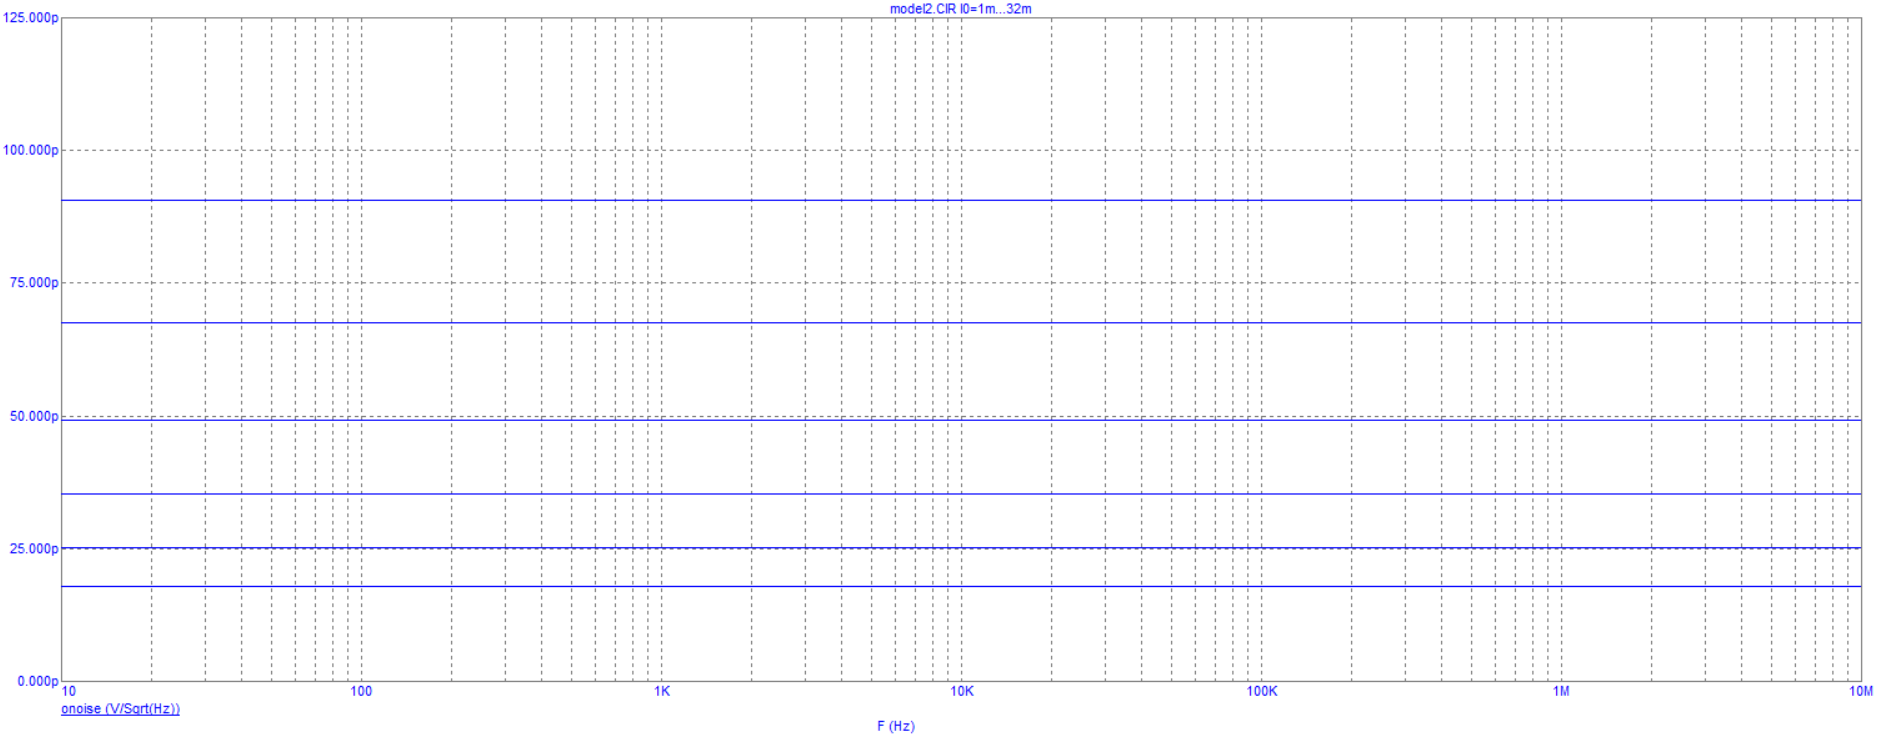
\includegraphics[scale=0.3]{images/mod2_1_2.png}
    \caption{Умеренные токи}
    \label{fig:m212}
\end{figure}

Для перевернутого диода поведение при низких токах будет идентично с точностью до значений(дробовой шум от направления не зависит). Напряжение пробоя диода измерим, пустив по нему большой ток(см рис, варьирование [1m, 32, log 2]). Пробой происходит при порядка 200 пА <-> 200 пВ.

\begin{figure}[h!]
    \centering
    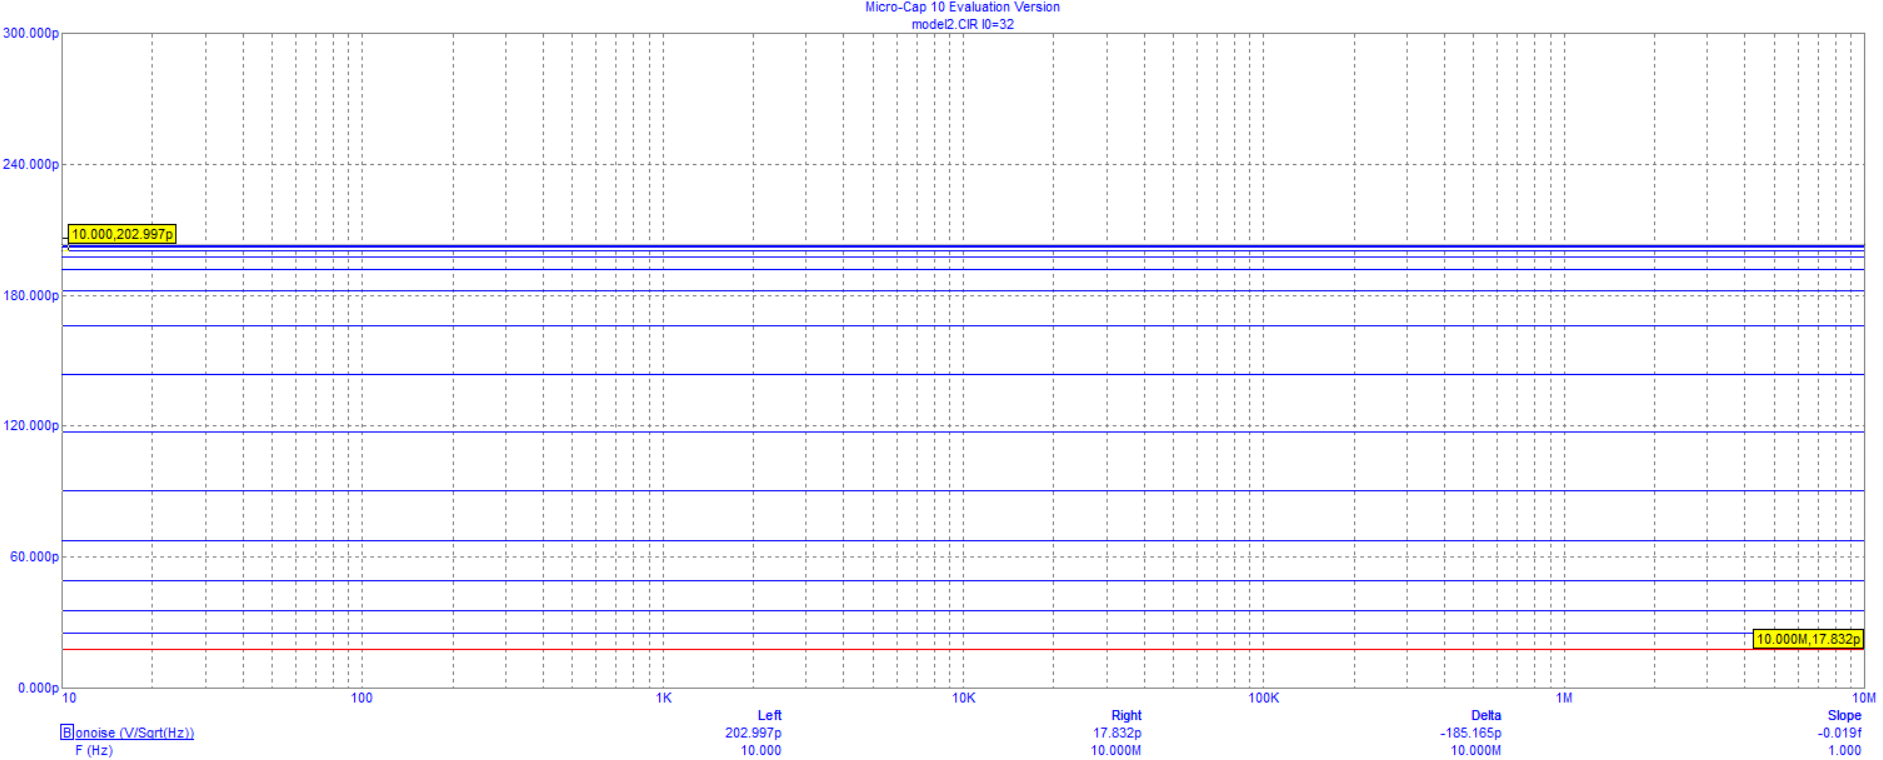
\includegraphics[scale=0.225]{images/cus_mod_2.png}
    \caption{Напряжение пробоя}
    \label{fig:m212}
\end{figure}


\item

Найдем $r_d$ как $r_d \approx K R_1$, $R_1 = 10k$:

\begin{itemize}
    \item $I_{01} = 1m$ => $K_{1} = 5.16m$ => $r_d = 51.6$ Ом;
    \item $I_{02} = 100\mu$ => $K_{2} = 49.24m$ => $r_d = 492.4$ Ом;
    \item $I_{03} = 10\mu$ => $K_{3} = 341.56m$ => $r_d \approx 3415.6$ Ом;
    \item $I_{04} = 1\mu$ => $K_{4} = 841.71m$ => $r_d \approx 8417.1$ Ом;
\end{itemize}

\begin{figure}[h!]
    \centering
    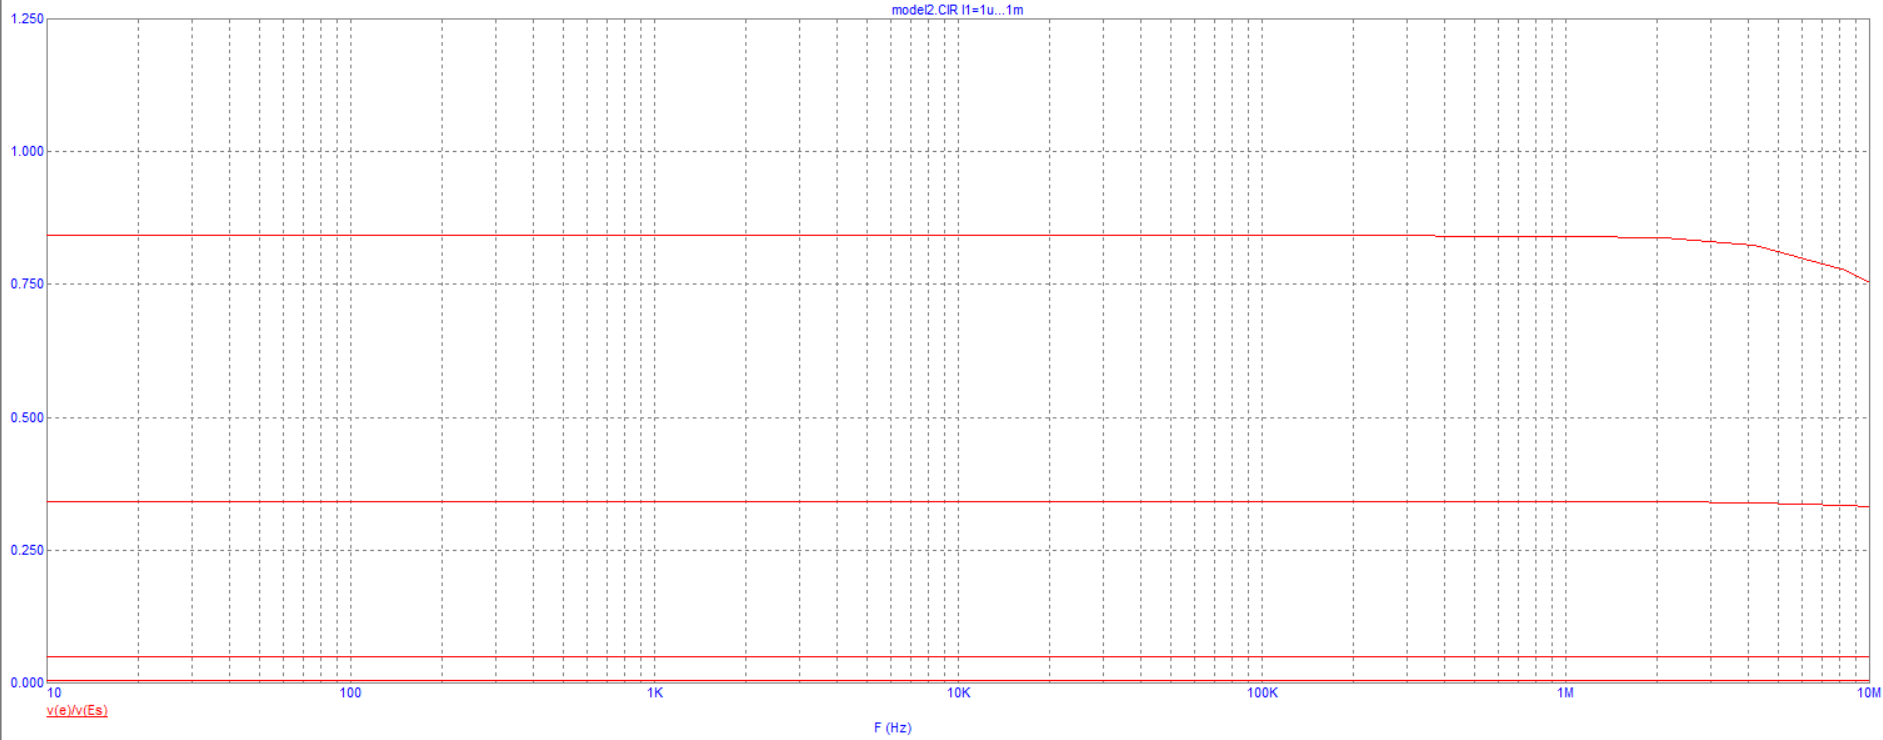
\includegraphics[scale=0.3]{images/mod2_2.png}
    \caption{$K = r_d/(R_1 + r_d)$}
    \label{fig:m212}
\end{figure}

\newpage

\item

\begin{figure}[h!]
    \centering
    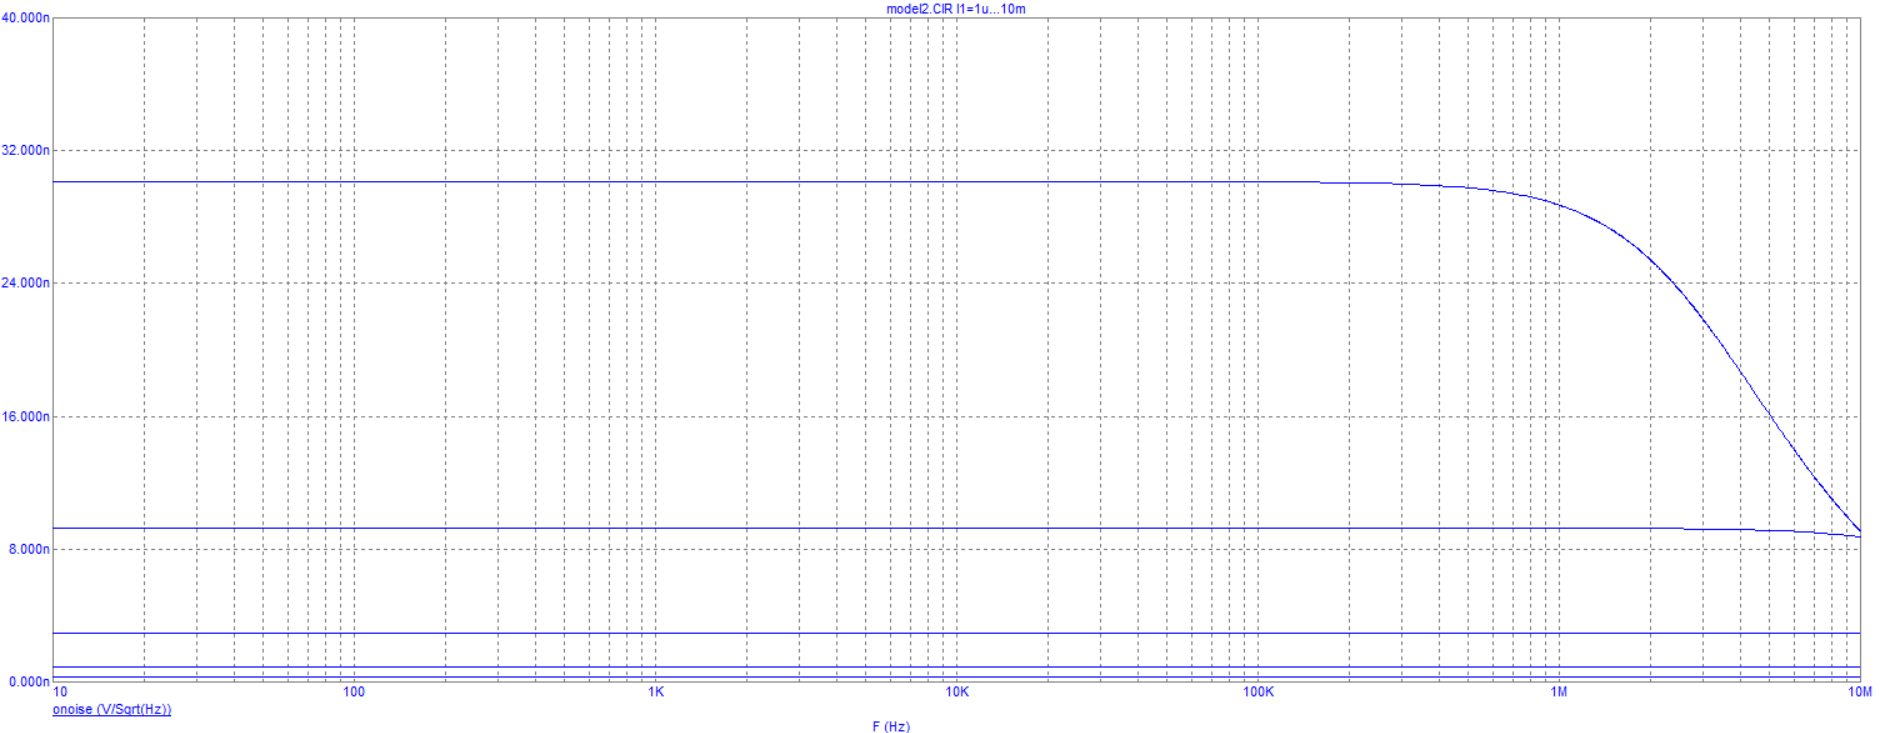
\includegraphics[scale=0.3]{images/mod2_3.png}
    \caption{e(f) для I = [1u, 10m|Log10]}
    \label{fig:m23}
\end{figure}

Проверим формулу $e(f) = i(f)r_d$, возьмем $i(f) = \sqrt{2*e*I_{0i}}$:
\begin{itemize}
    \item $I_{01} = 1\mu$ => $e(f)_\text{теор} = 29.2n$, $e(f)_\text{прак} = 30.1n$;
    \item $I_{02} = 10\mu$ => $e(f)_\text{теор} = 8.8n$, $e(f)_\text{прак} = 9.3n$;
    \item $I_{03} = 100\mu$ => $e(f)_\text{теор} = 2.7n$, $e(f)_\text{прак} = 2.9n$;
    \item $I_{04} = 1m$ => $e(f)_\text{теор} = 1005p$, $e(f)_\text{прак} = 928p$;
    \item $I_{05} = 10m$ => $e(f)_\text{теор} = 410p$, $e(f)_\text{прак} = 304p$;
\end{itemize}

\item

Установим диод в режим пробоя и измерим максимальное шумовое напряжение на невысоких частотах. Оно составит 163 нВ. Ток $I_1$ составит 7.4 нА.

.

\begin{figure}[h!]
    \centering
    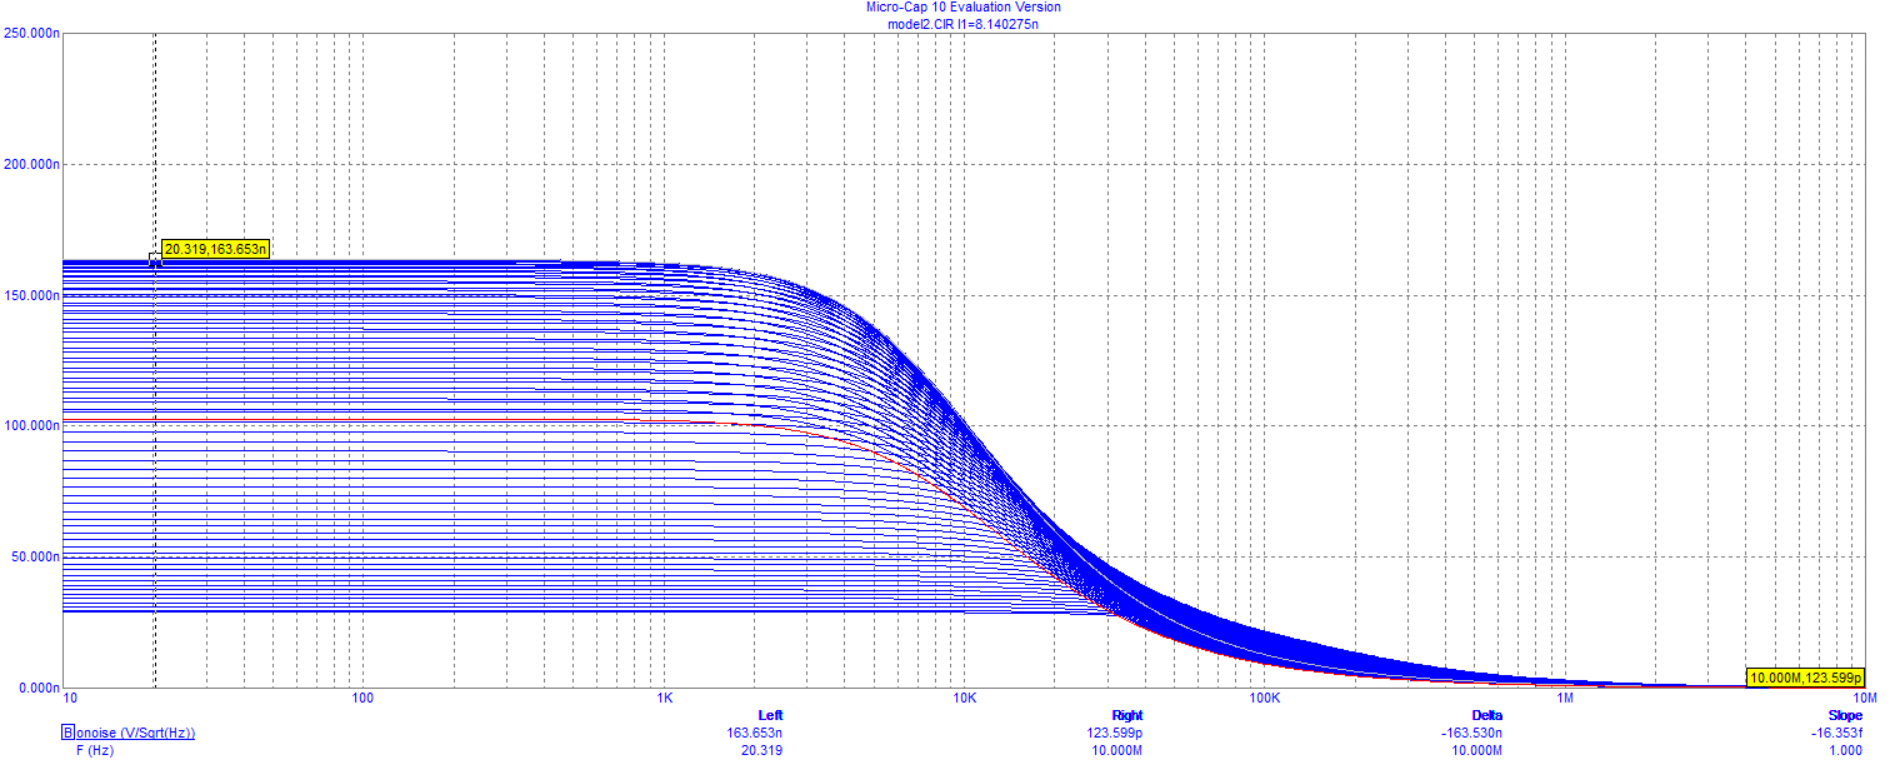
\includegraphics[scale=0.225]{images/cus_mod_2_1.png}
    \caption{e(f) для I = [1n, 1u|Log1.1]}
    \label{fig:m23}
\end{figure}

уровень же шума $\sigma$ примет следующую зависимость от частоты

\begin{figure}[h!]
    \centering
    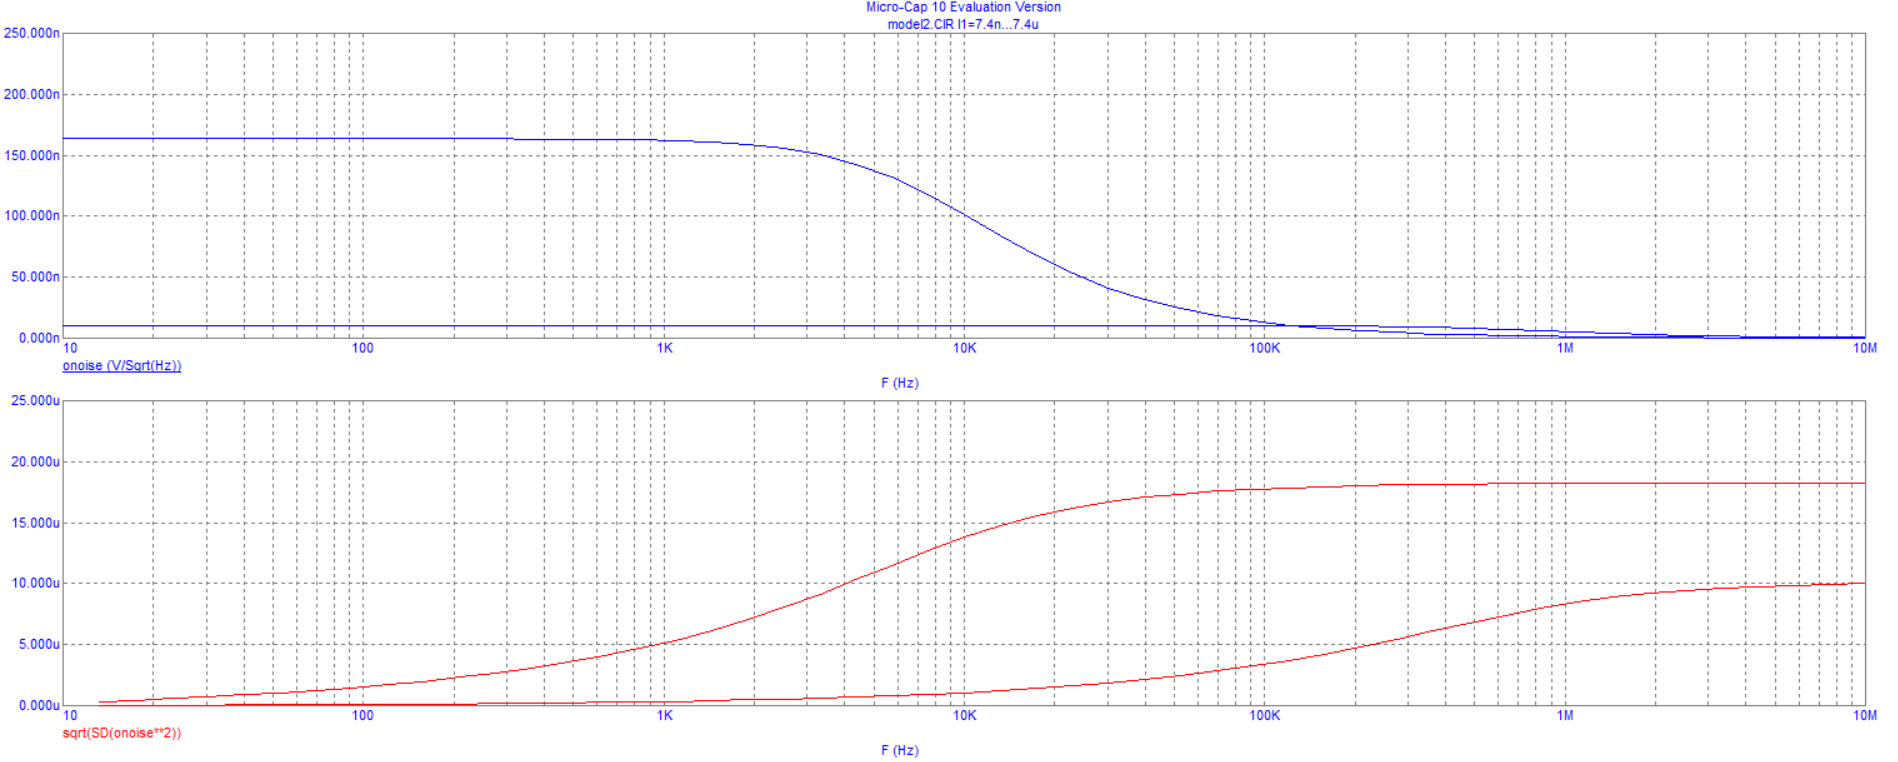
\includegraphics[scale=0.225]{images/cus_mod_2_2.png}
    \caption{$\sigma$(f) для I1 = 7.4}
    \label{fig:m23}
\end{figure}

\end{enumerate}

\newpage

\section{\textbf{model 3 (Фильтрация шумов)}}

\subsection*{Интегрирующая цепь}

\begin{enumerate}

\item

\begin{figure}[h!]
    \centering
    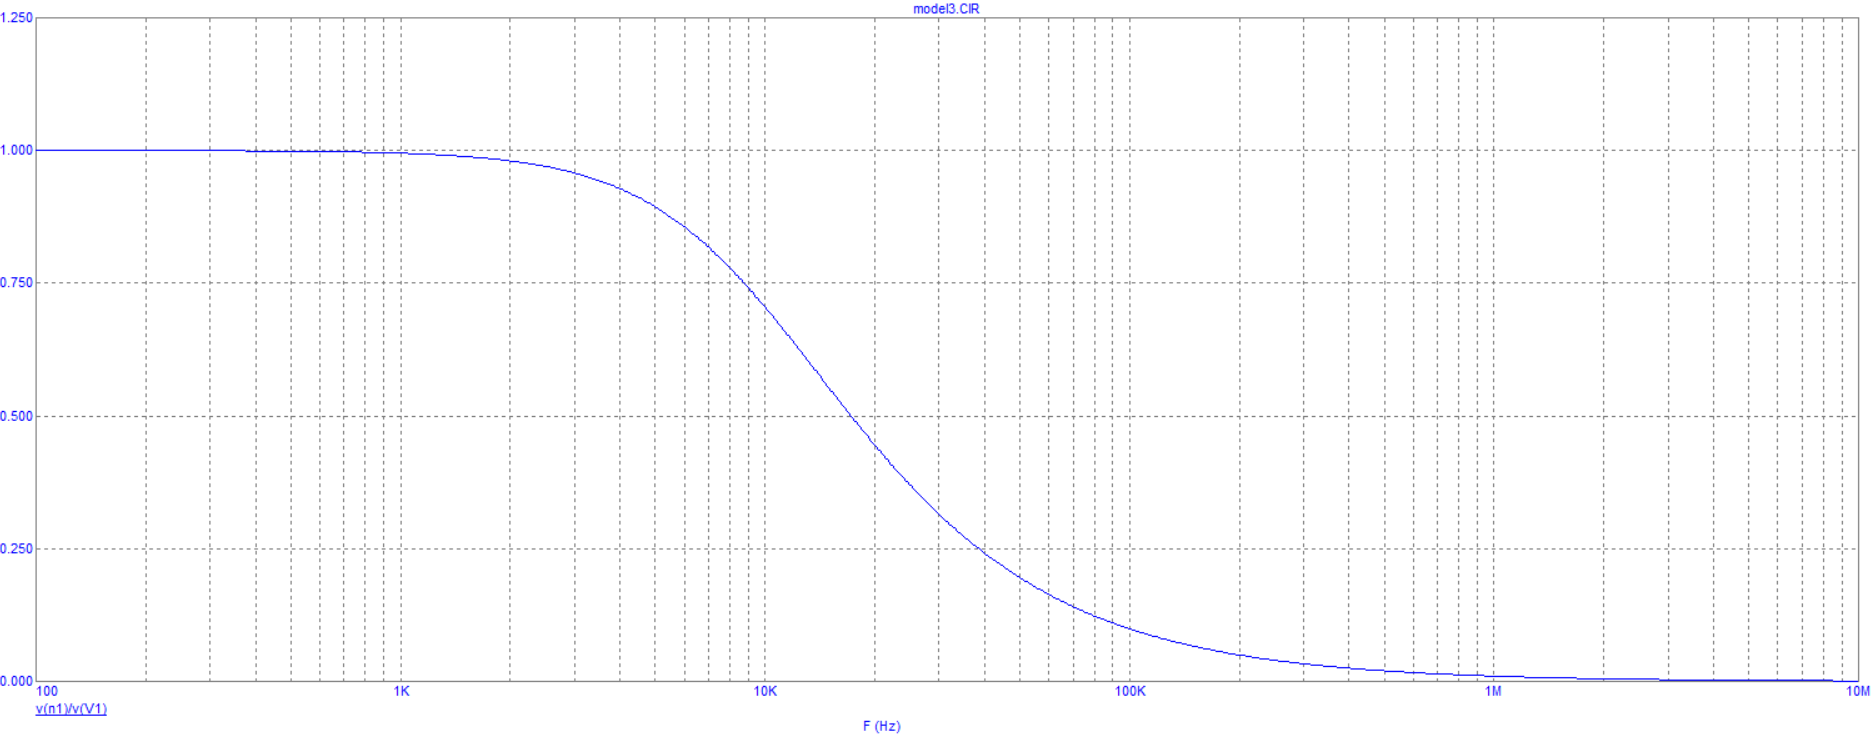
\includegraphics[scale=0.3]{images/mod3_1_1.png}
    \caption{Граничная частота составляет $f_h = 10$ кГц}
    \label{fig:m311}
\end{figure}

$\sigma_\text{теор1} = n_1\sqrt{Fn} = 12.8n\sqrt{\pi/2 \cdot 10000} = 1.63\mu \approx \sigma_\text{теор2} = \sqrt{\frac{kT}{C}} = 1.61\mu$

$\sigma_\text{прак} = 1.60\mu$

\begin{figure}[h!]
    \centering
    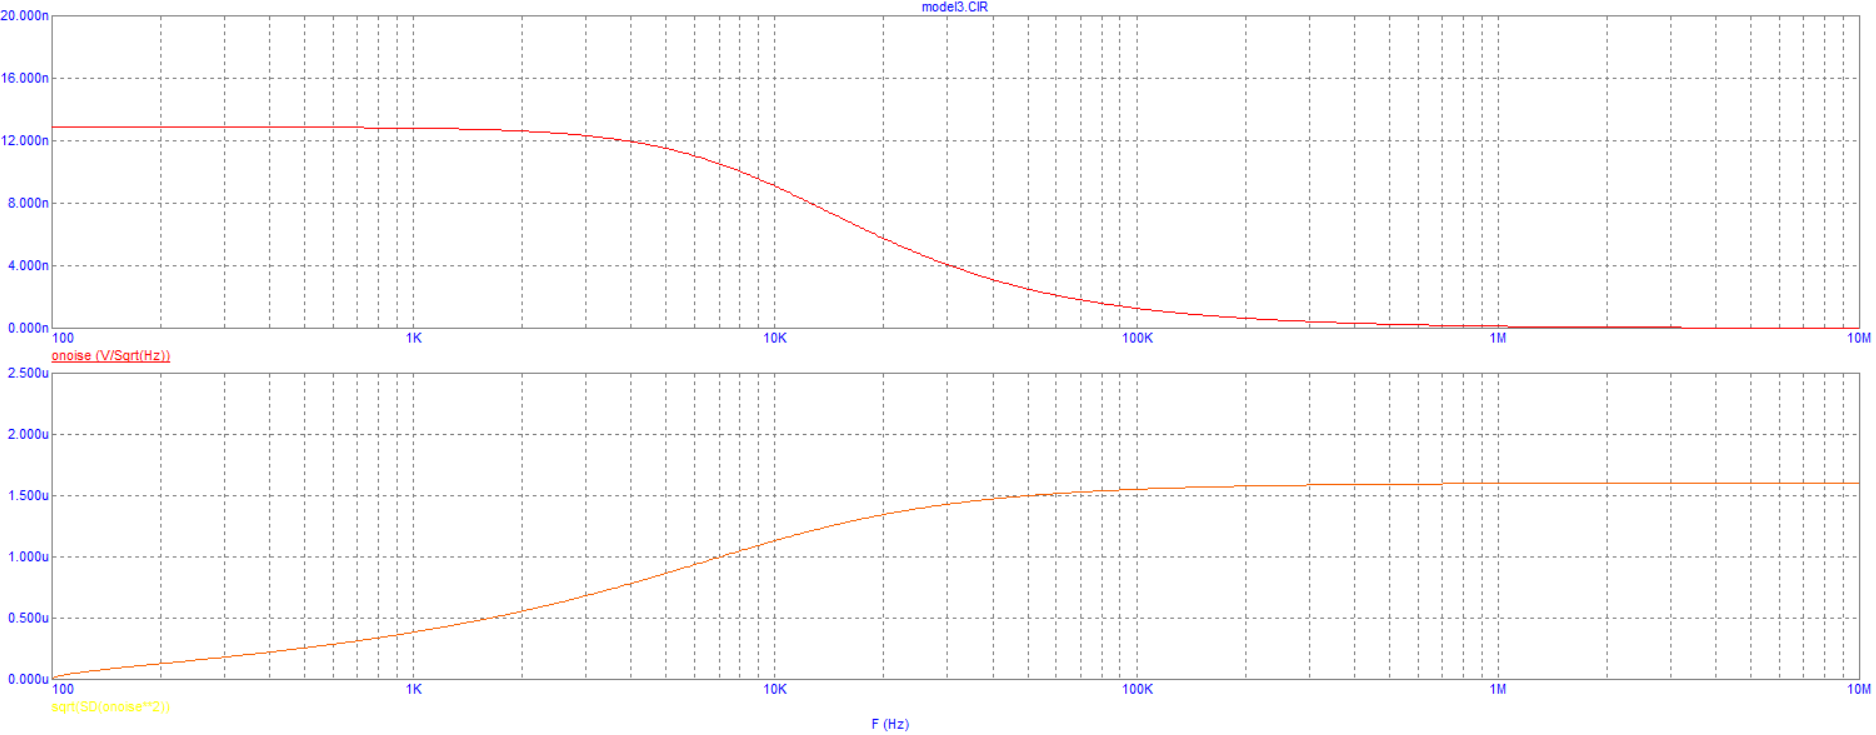
\includegraphics[scale=0.3]{images/mod3_1_2.png}
    \caption{Уровень шума}
    \label{fig:m312}
\end{figure}

\newpage

Снимем зависимость шумового напряжения от $R_1$:
\begin{itemize}
    \item $R_1 = 2k => n_1(f) = 5.8n$;
    \item $R_1 = 6k => n_1(f) = 10n$;
    \item $R_1 = 10k => n_1(f) = 12.8n$;
    \item $R_1 = 14k => n_1(f) = 15.6n$;
    \item $R_1 = 16k => n_1(f) = 16.3n$;
\end{itemize}

Уровень шума на выходе не зависит от $R_1$, поскольку шум создает резистор, а значит $\sigma = \sqrt{P} = \sqrt{\frac{kT}{C}}$ от R не зависит

\begin{figure}[h!]
    \centering
    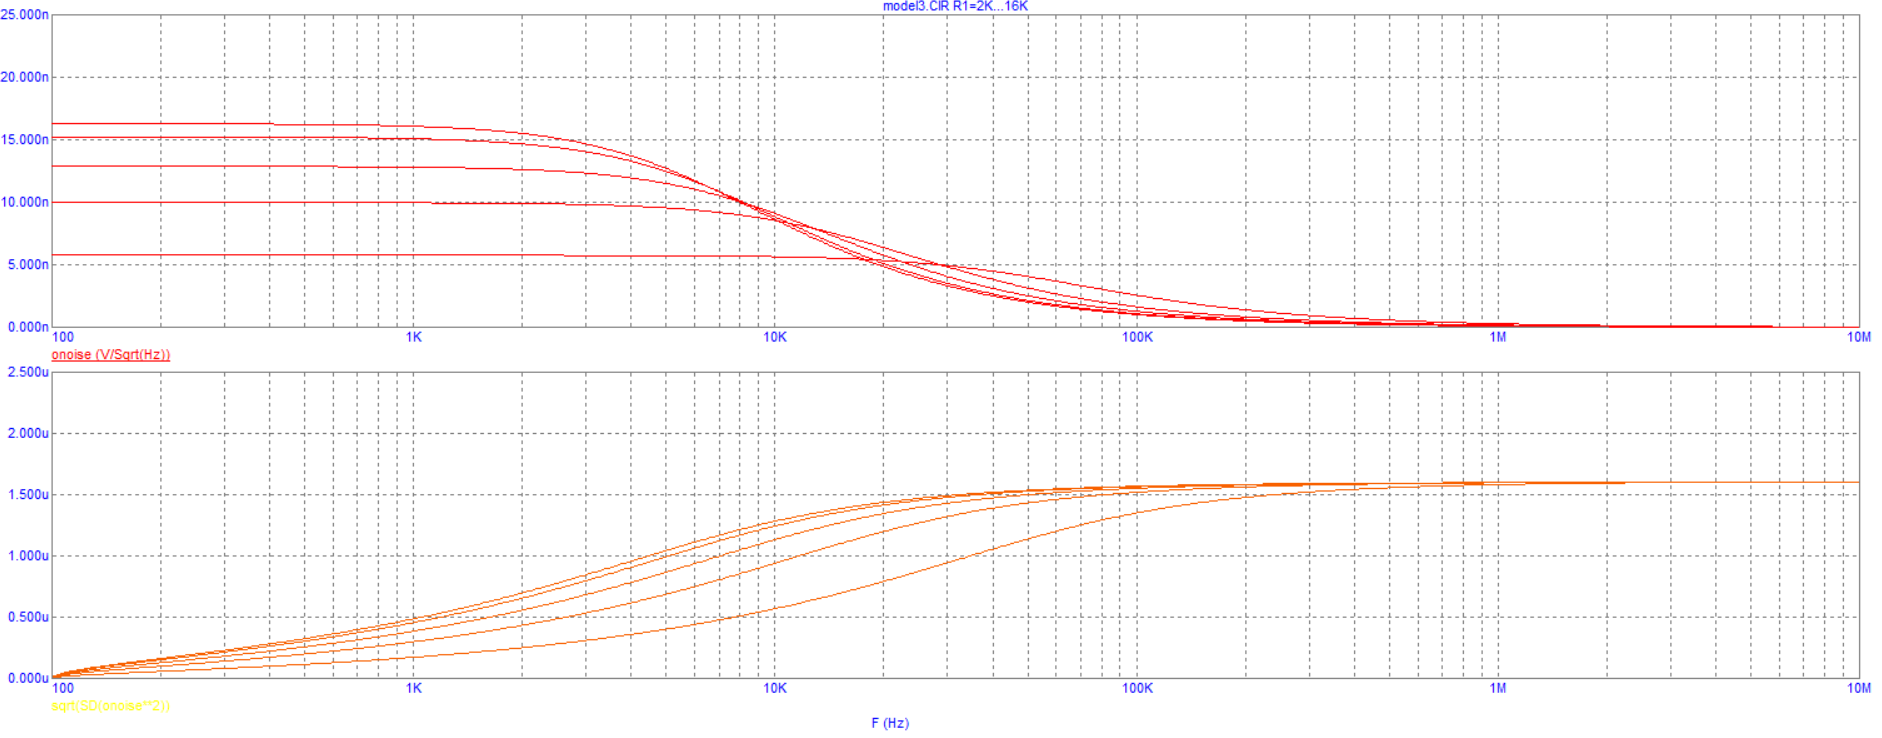
\includegraphics[scale=0.3]{images/mod3_1_3.png}
    \caption{Варьирование $R_1$ = [2k, 16k|4k]}
    \label{fig:m313}
\end{figure}

Снимем зависимость уровня шума от $C_1$:
\begin{itemize}
    \item $C_1 = 0.8k => n_1(f) = 2.27\mu$;
    \item $C_1 = 1.2k => n_1(f) = 1.85\mu$;
    \item $C_1 = 1.6k => n_1(f) = 1.60\mu$;
    \item $C_1 = 2.0k => n_1(f) = 1.44\mu$;
    \item $C_1 = 2.4k => n_1(f) = 1.31\mu$;
\end{itemize}

\begin{figure}[h!]
    \centering
    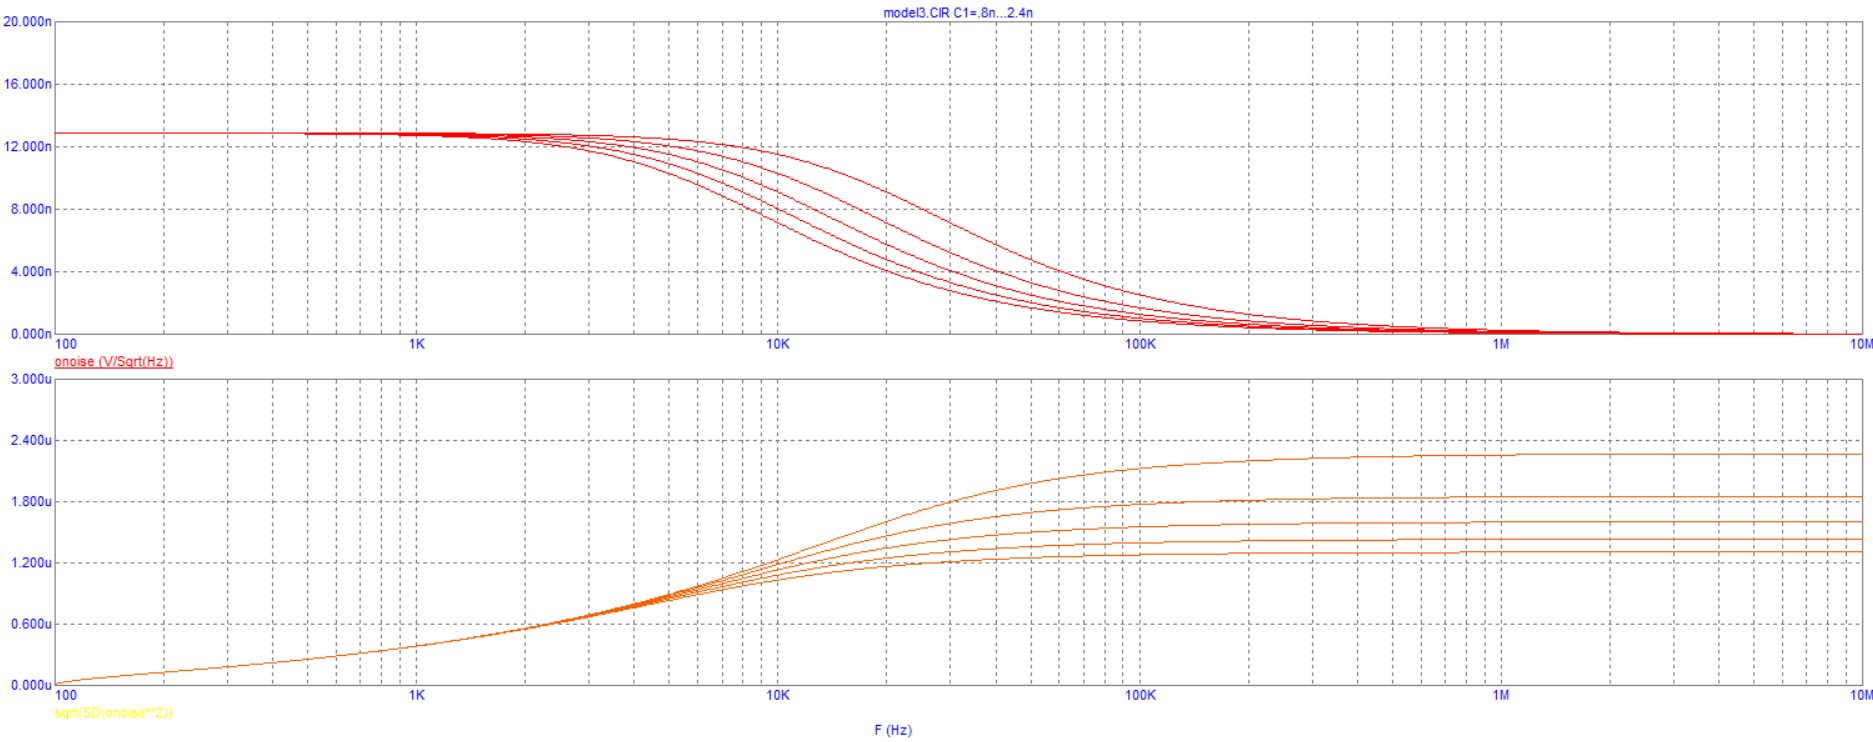
\includegraphics[scale=0.3]{images/mod3_1_4.png}
    \caption{Варьирование $C_1$ = [0.8n, 2.4n|0.4n]}
    \label{fig:m314}
\end{figure}


\end{enumerate}

\subsection*{Полосовой LC-фильтр}

\begin{enumerate}

\item

.

\begin{figure}[h!]
    \centering
    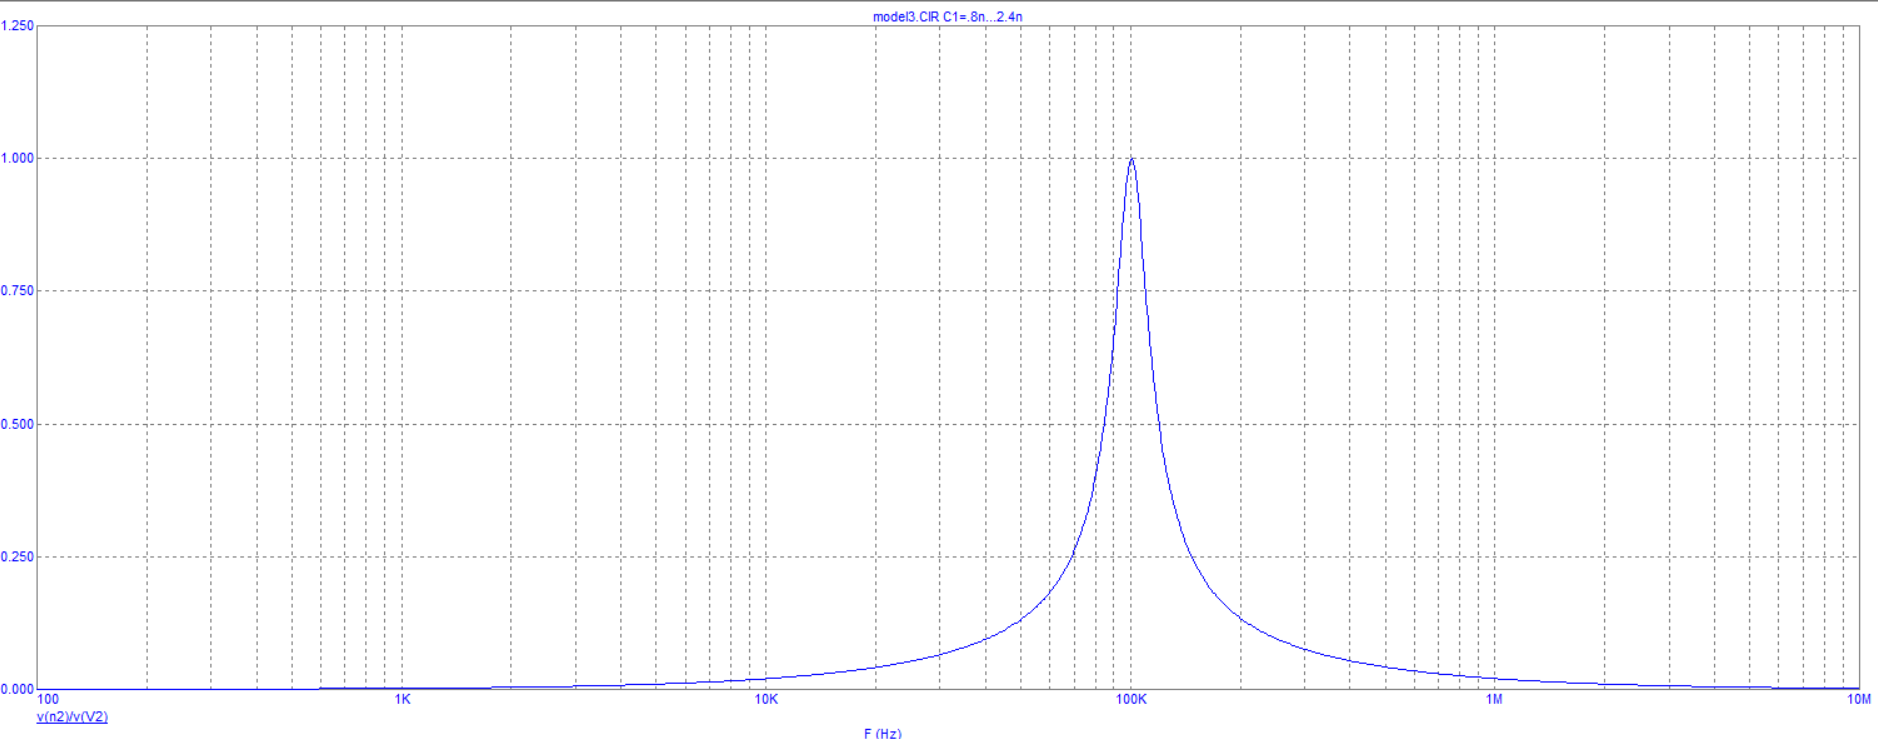
\includegraphics[scale=0.3]{images/mod3_2_1.png}
    \caption{$f_0 = 100k, \Delta f = 20k$, Q = 5}
    \label{fig:m321}
\end{figure}


\item

.

\begin{figure}[h!]
    \centering
    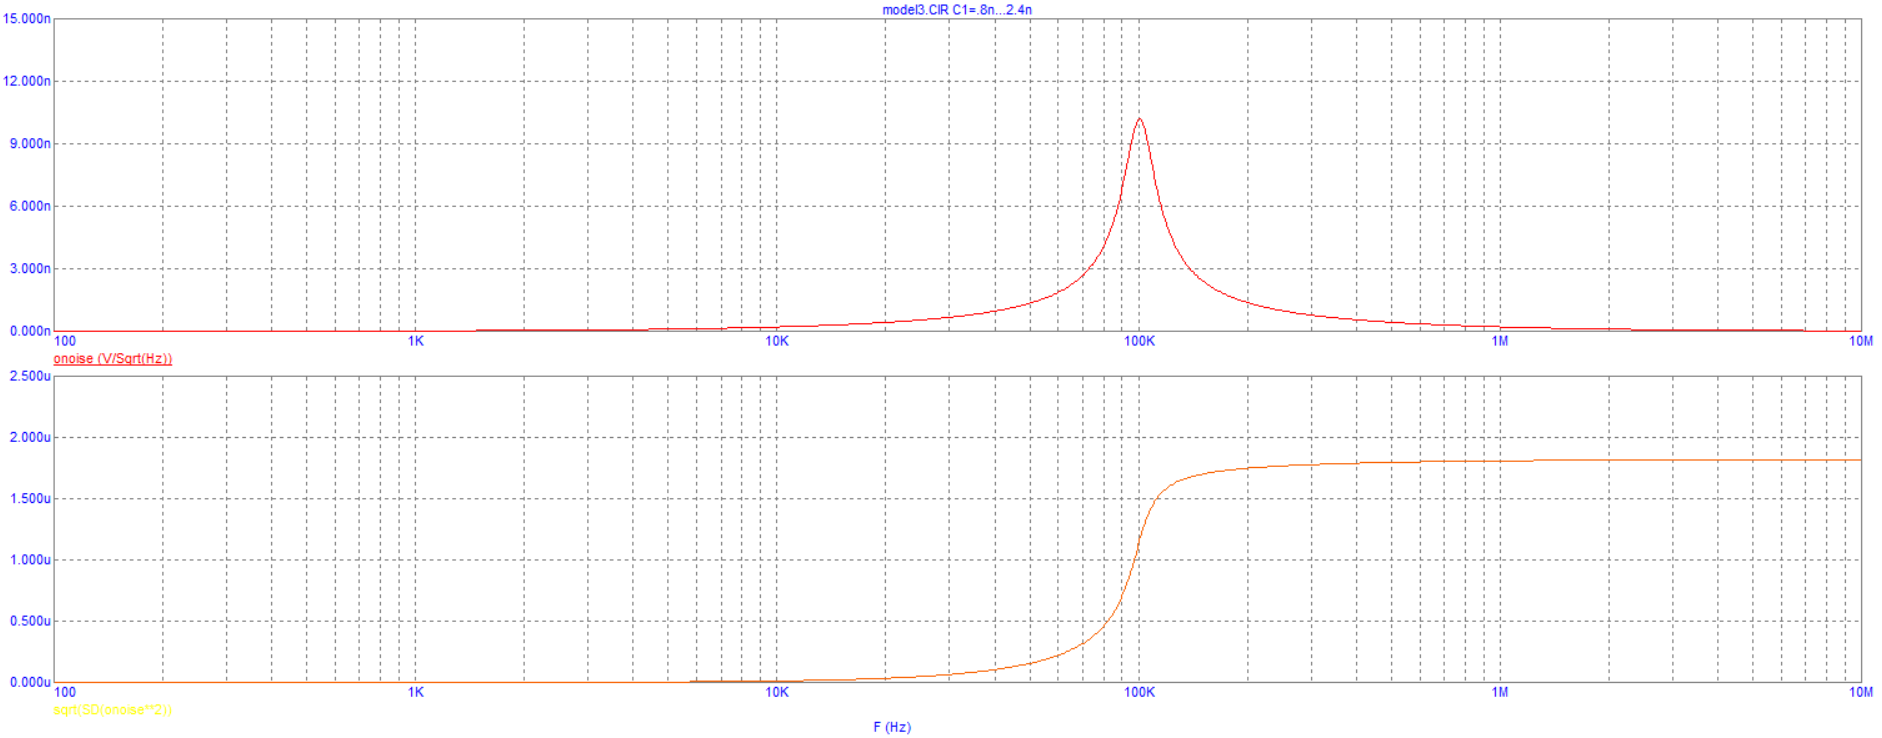
\includegraphics[scale=0.3]{images/mod3_2_2.png}
    \caption{$n_2(f_0) = 10n, \sigma = 1.82\mu$}
    \label{fig:m322}
\end{figure}

Проверим формулу $\sigma = n_2\sqrt{F_n} = \sqrt{\frac{kT}{C}} = 1.80$, формула работает.

\item

.

\begin{figure}[h!]
    \centering
    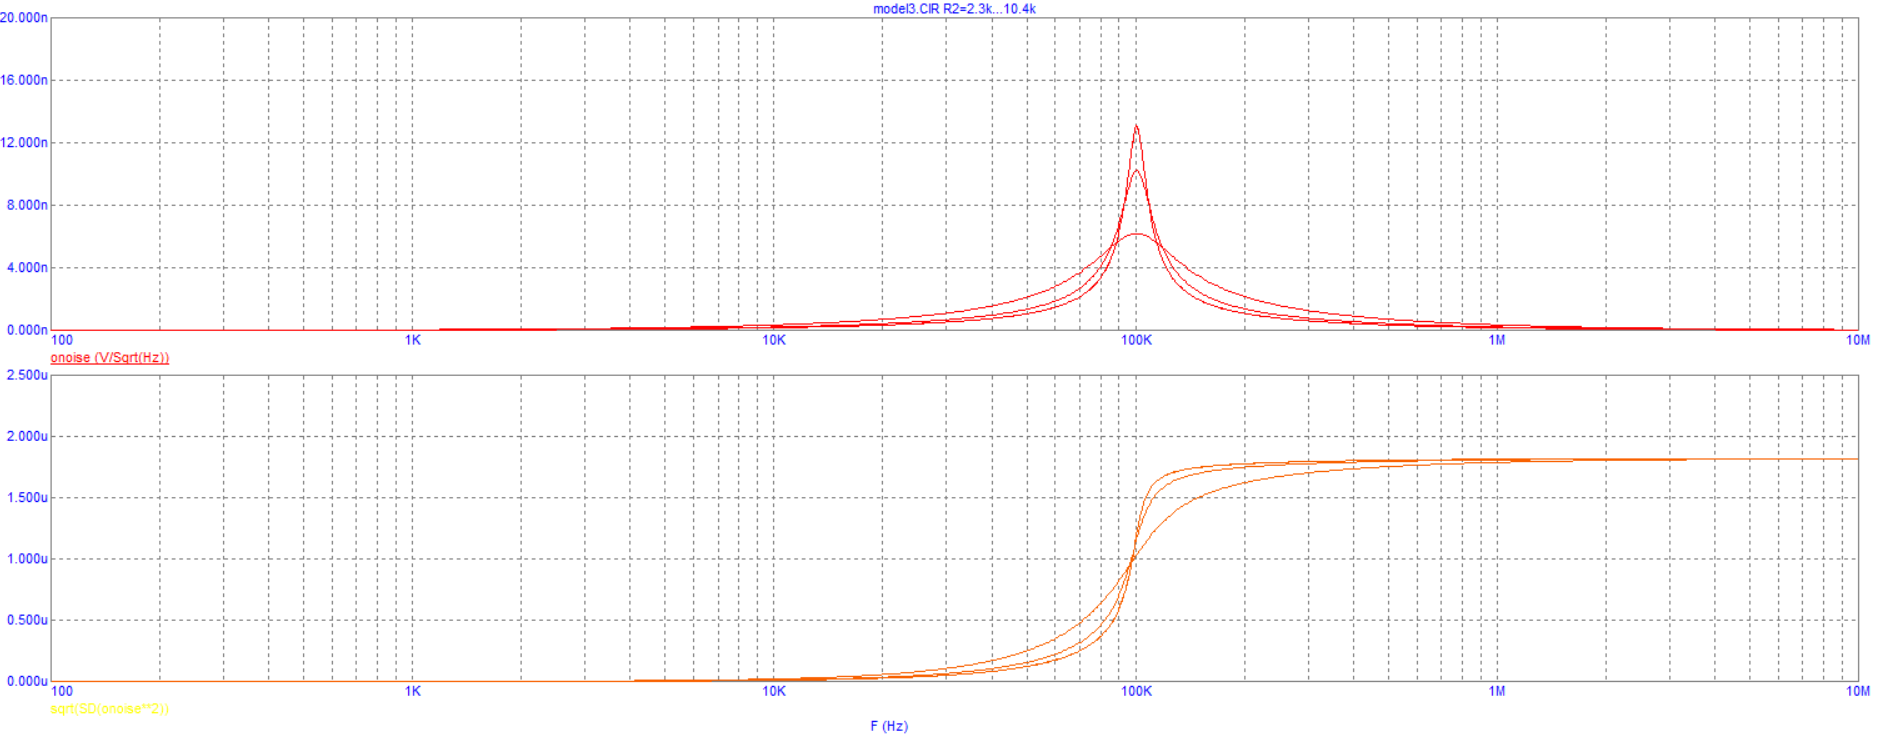
\includegraphics[scale=0.3]{images/mod3_2_3.png}
    \caption{Варьирование $R_2$ = [2.3k, 10.3k|4k]}
    \label{fig:m323}
\end{figure}

Зависимость $n_2(f_0)$ от $R_2$:
\begin{itemize}
    \item $R_2 = 2.3k => n_2 = 6.08n$;
    \item $R_2 = 6.3k => n_2 = 10.08$;
    \item $R_2 = 10.3k => n_2 = 13.04$;
\end{itemize}

Уровень шума на выходе не зависит по той-же самой причине, формула для $\sigma = \sqrt{\frac{kT}{C}}$

\item

.

\begin{figure}[h!]
    \centering
    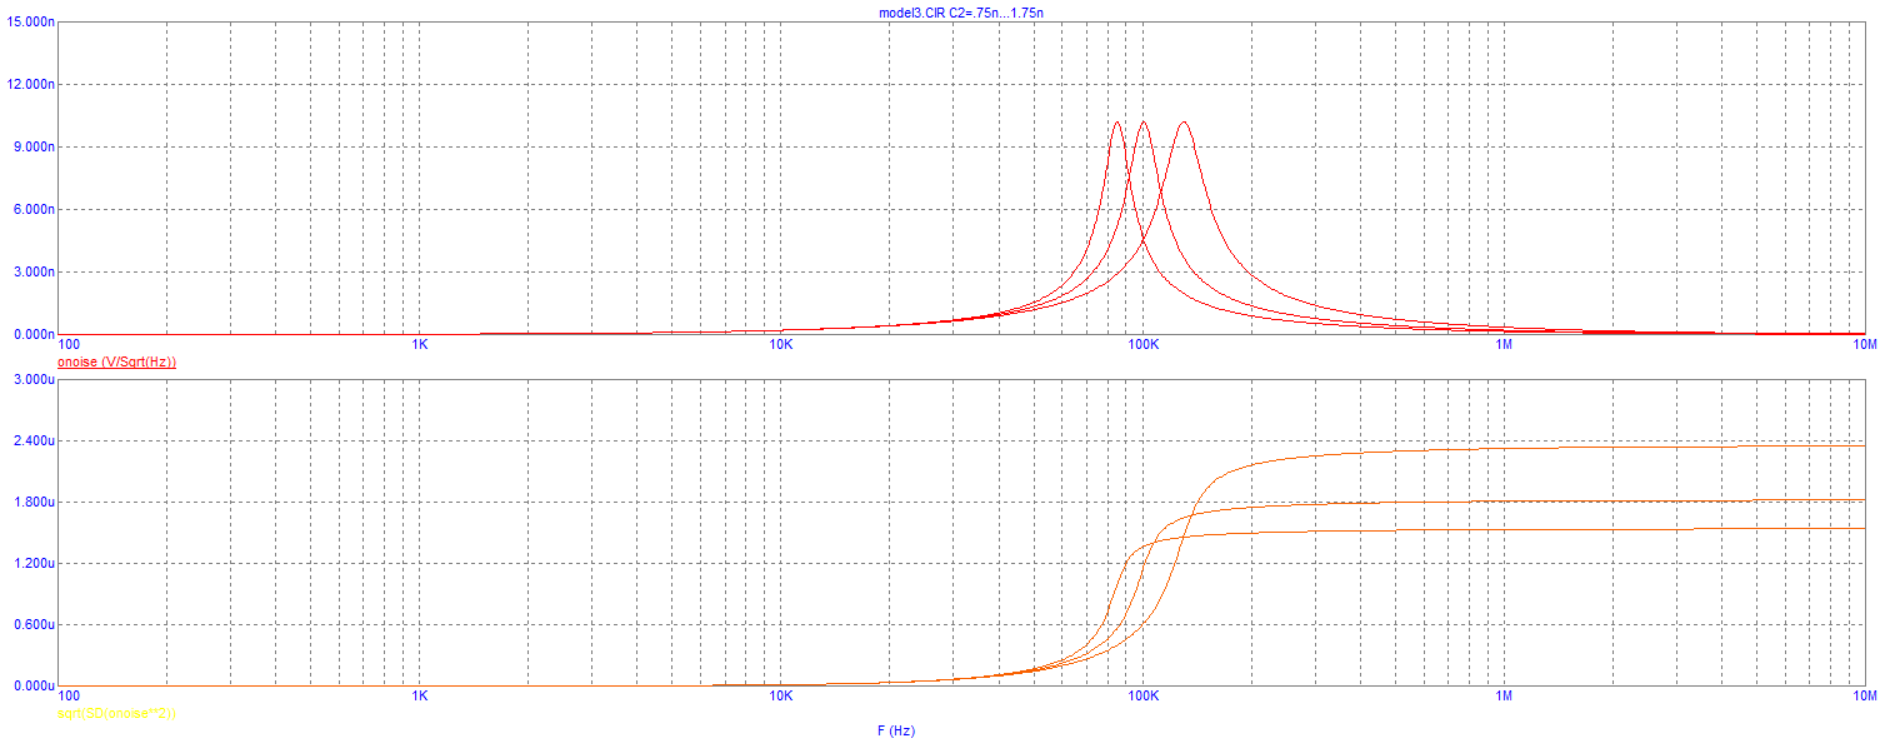
\includegraphics[scale=0.3]{images/mod3_2_4.png}
    \caption{Варьирование $C_2$ = [0.75n, 1.75n|0.5n]}
    \label{fig:m324}
\end{figure}

Зависимость $\sigma$ от $C_2$:
\begin{itemize}
    \item $C_2 = 0.75n => \sigma = 2.34\mu$;
    \item $C_2 = 1.25n => \sigma = 1.82\mu$;
    \item $C_2 = 1.75n => \sigma = 1.52\mu$;
\end{itemize}

\item

.

\begin{figure}[h!]
    \centering
    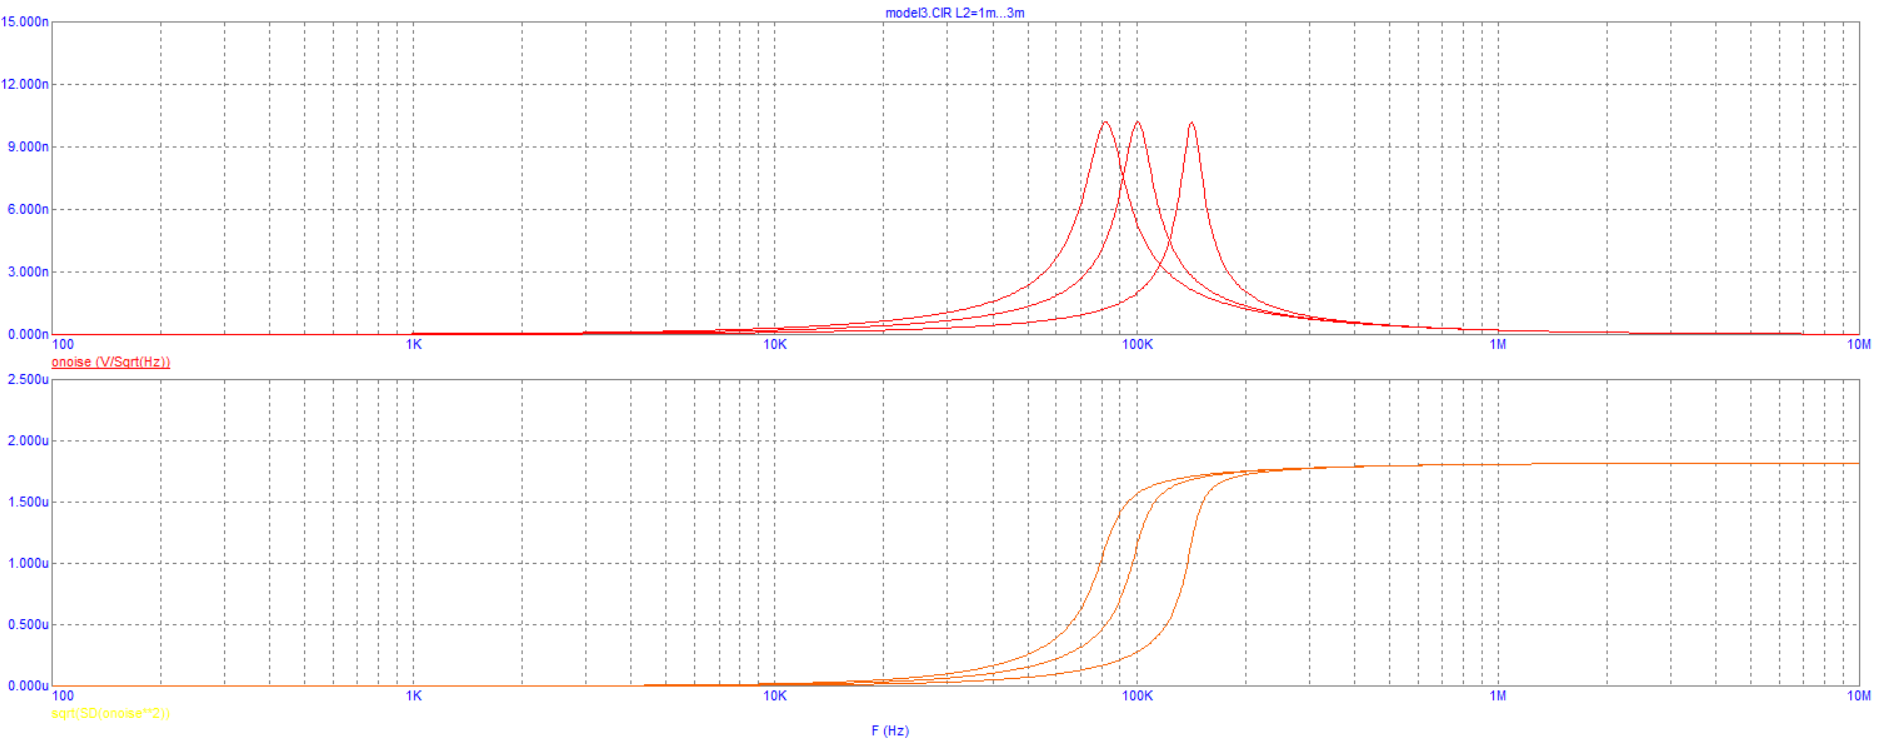
\includegraphics[scale=0.3]{images/mod3_2_5.png}
    \caption{Варьирование $L_2$ = [1m, 3m|1m]}
    \label{fig:m325}
\end{figure}

Уровень шума на выходе не зависит от индуктивности по формуле для $\sigma = \sqrt{\frac{kT}{C}}$.

\end{enumerate}

\subsection*{LC-фильтр нижних частот}

\begin{enumerate}	

\item

Характеристики: $K(p) = \frac{1}{p^2+2 \delta p + 1}, p = \frac{j f}{f_0}, f_0 = 100 k, \rho = 1260, Q = \frac{1}{2 \delta} = 5$

\newpage	

\begin{figure}[h!]
    \centering
    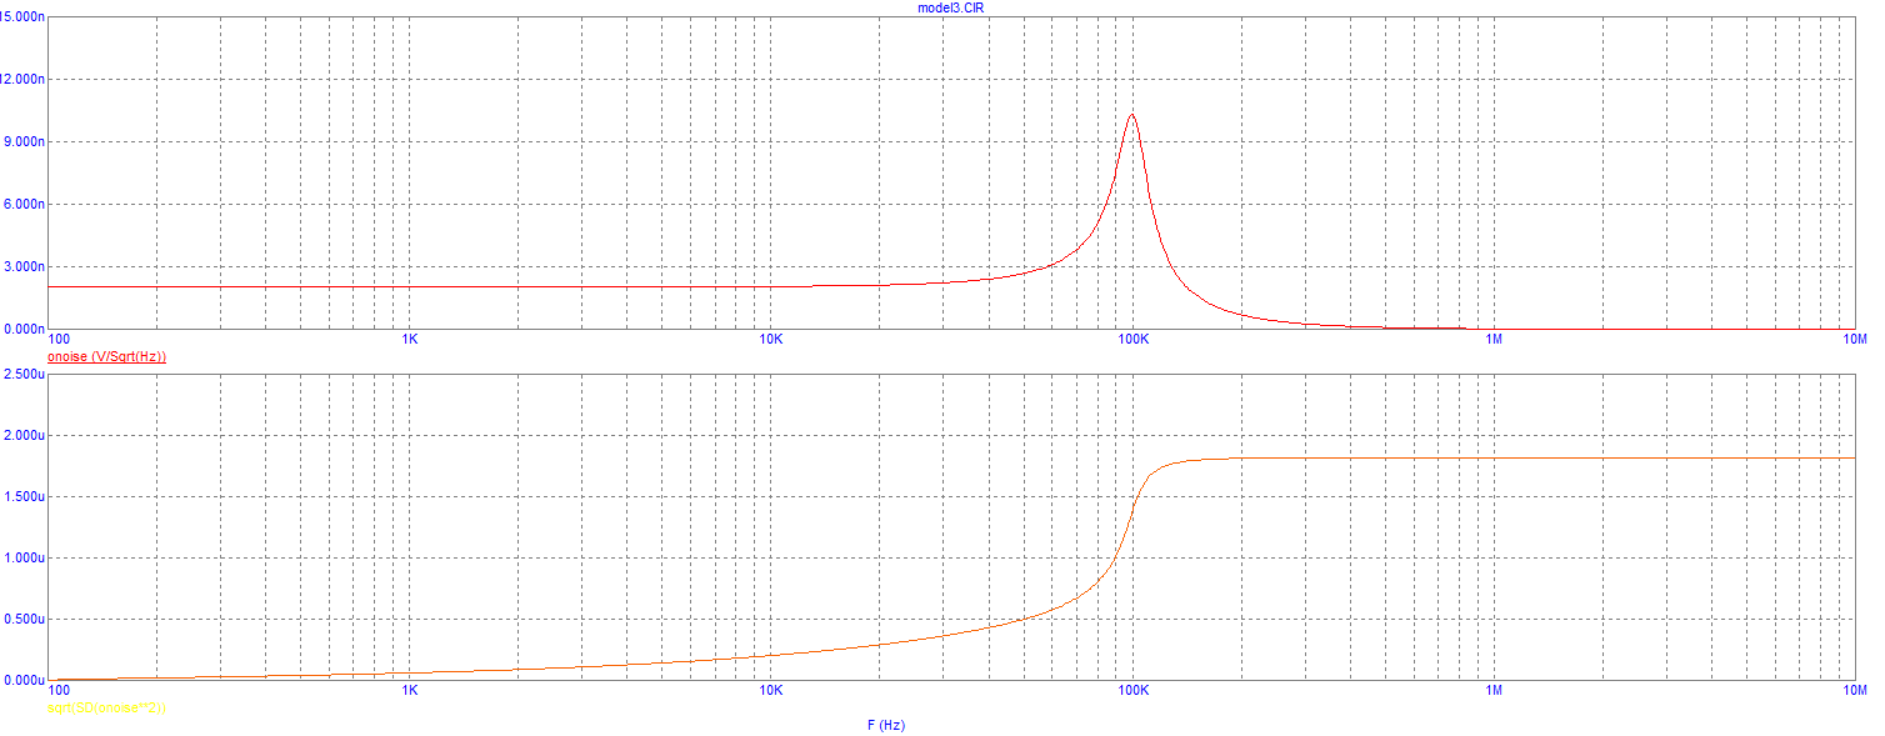
\includegraphics[scale=0.3]{images/mod3_3_1.png}
    \caption{$n_3(f_0) = 10.2n, n_3(f_0/10) = 2.05n, \sigma = 1.82\mu$}
    \label{fig:m331}
\end{figure}

Разумеется значение $n_3$ будет совпадать с шумовым напряжением резистора, поскольку при низких частотах фильтр себя не проявляет(конденсатор - обрыв, катушка - провод) и весь шум идет от резистора на узел n3.

Оценим шумовую полосу $F_{n\text{теор}} = \frac{\pi}{2}\frac{f_0}{Q} = 31k, F_{n\text{прак}} = 30.9k$

\begin{figure}[h!]
    \centering
    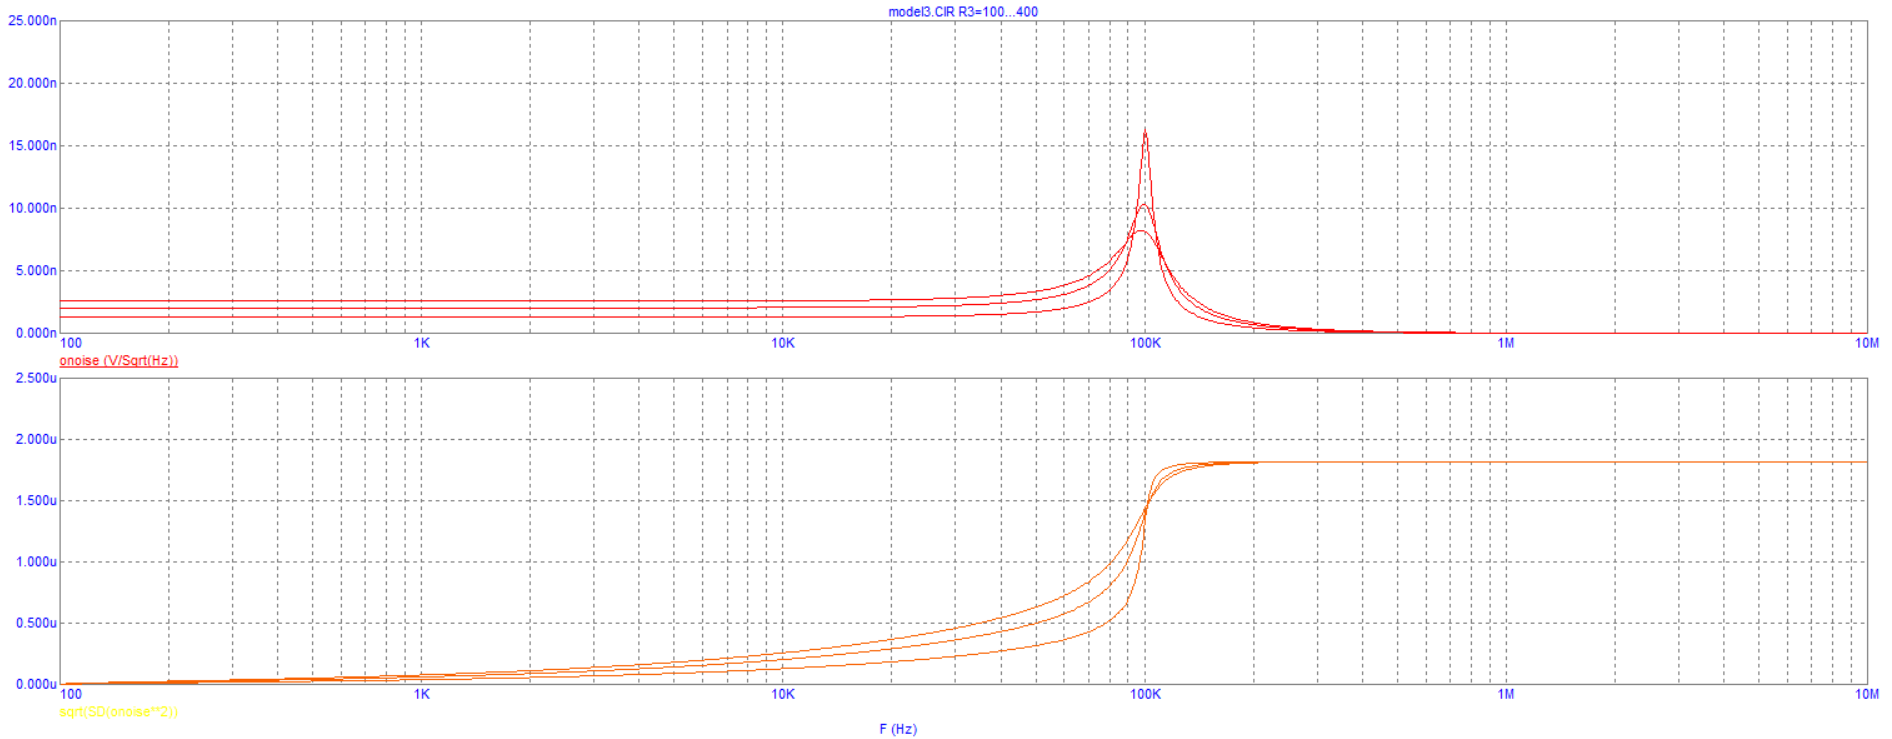
\includegraphics[scale=0.3]{images/mod3_3_2_1.png}
    \caption{Варьирование R3 = [100,400|150]}
    \label{fig:m3321}
\end{figure}

\begin{center}
\begin{tabular}{|c|c|c|c|}
\hline
    R3 & 400 & 250 & 100\\ \hline
    $n_3(f_0)$ & 8.1n & 10.3n & 15.9n\\ \hline
    $n_3(f_0/10)$ & 1.1n & 2n & 2.6n\\ \hline
    $\sigma$ & 1.8$\mu$ & 1.8$\mu$ & 1.8$\mu$\\ \hline
\end{tabular}
\end{center}

\newpage

\begin{figure}[h!]
    \centering
    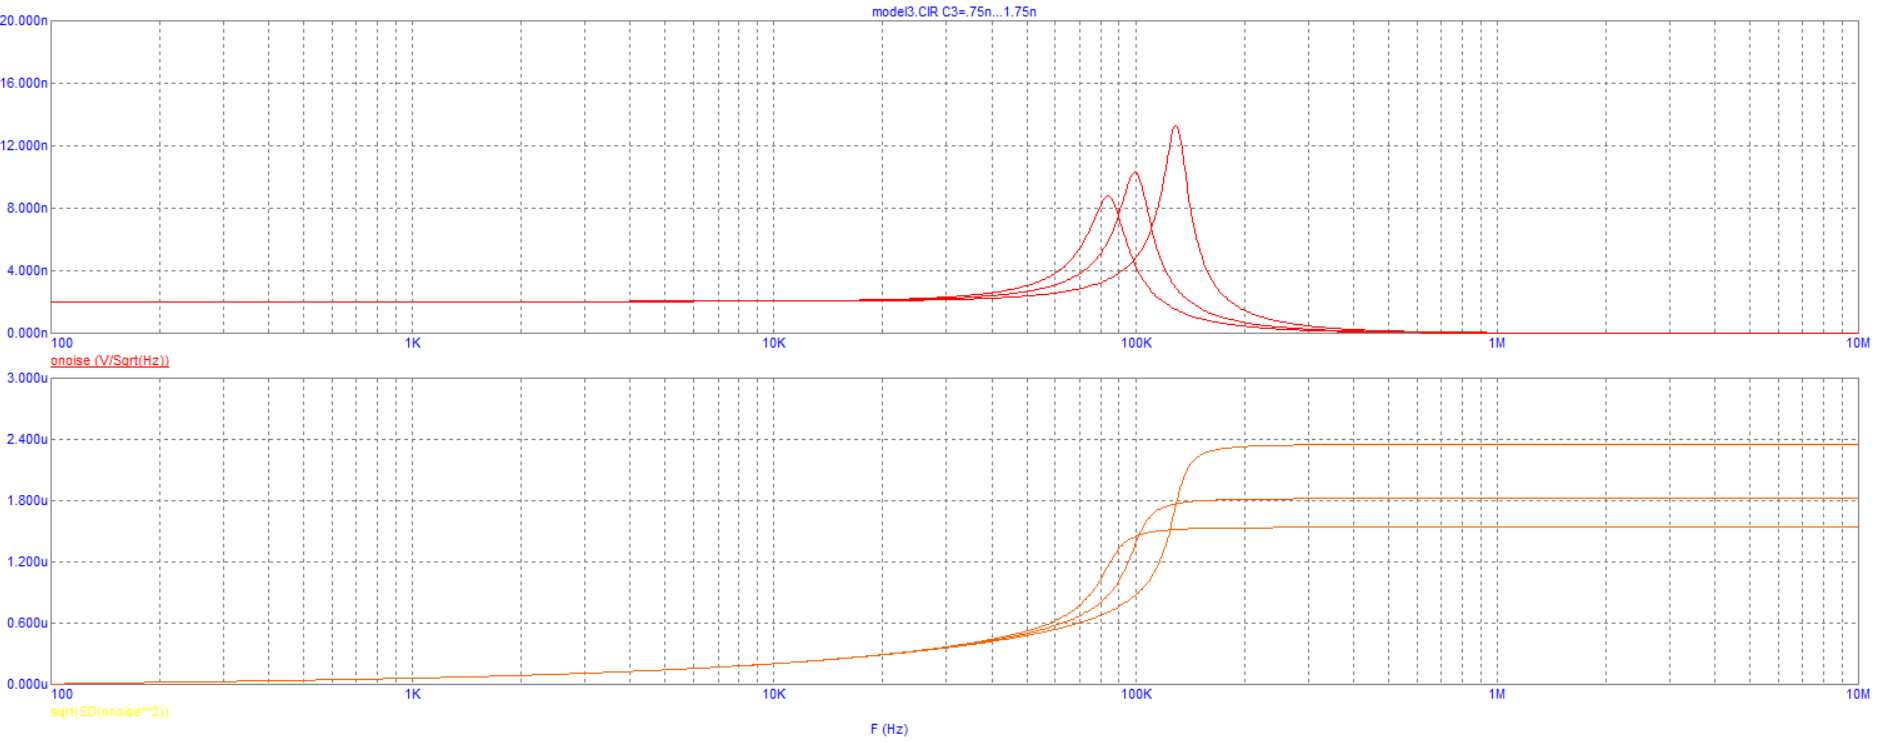
\includegraphics[scale=0.3]{images/mod3_3_2_2.png}
    \caption{Варьирование C3 = [0.75n, 1.75n |0.5n]}
    \label{fig:m3322}
\end{figure}

\begin{center}
\begin{tabular}{|c|c|c|c|}
\hline
    C3 & 0.75n & 1.25n & 1.75n\\ \hline
    $n_3(f_0)$ & 13.2n & 10.2n & 8.8n\\ \hline
    $n_3(f_0/10)$ & 2.1n & 2.1n & 2.1n \\ \hline
    $\sigma$ & 2.4$\mu$ & 1.8$\mu$ & 1.5$\mu$ \\ \hline
\end{tabular}
\end{center}

\begin{figure}[h!]
    \centering
    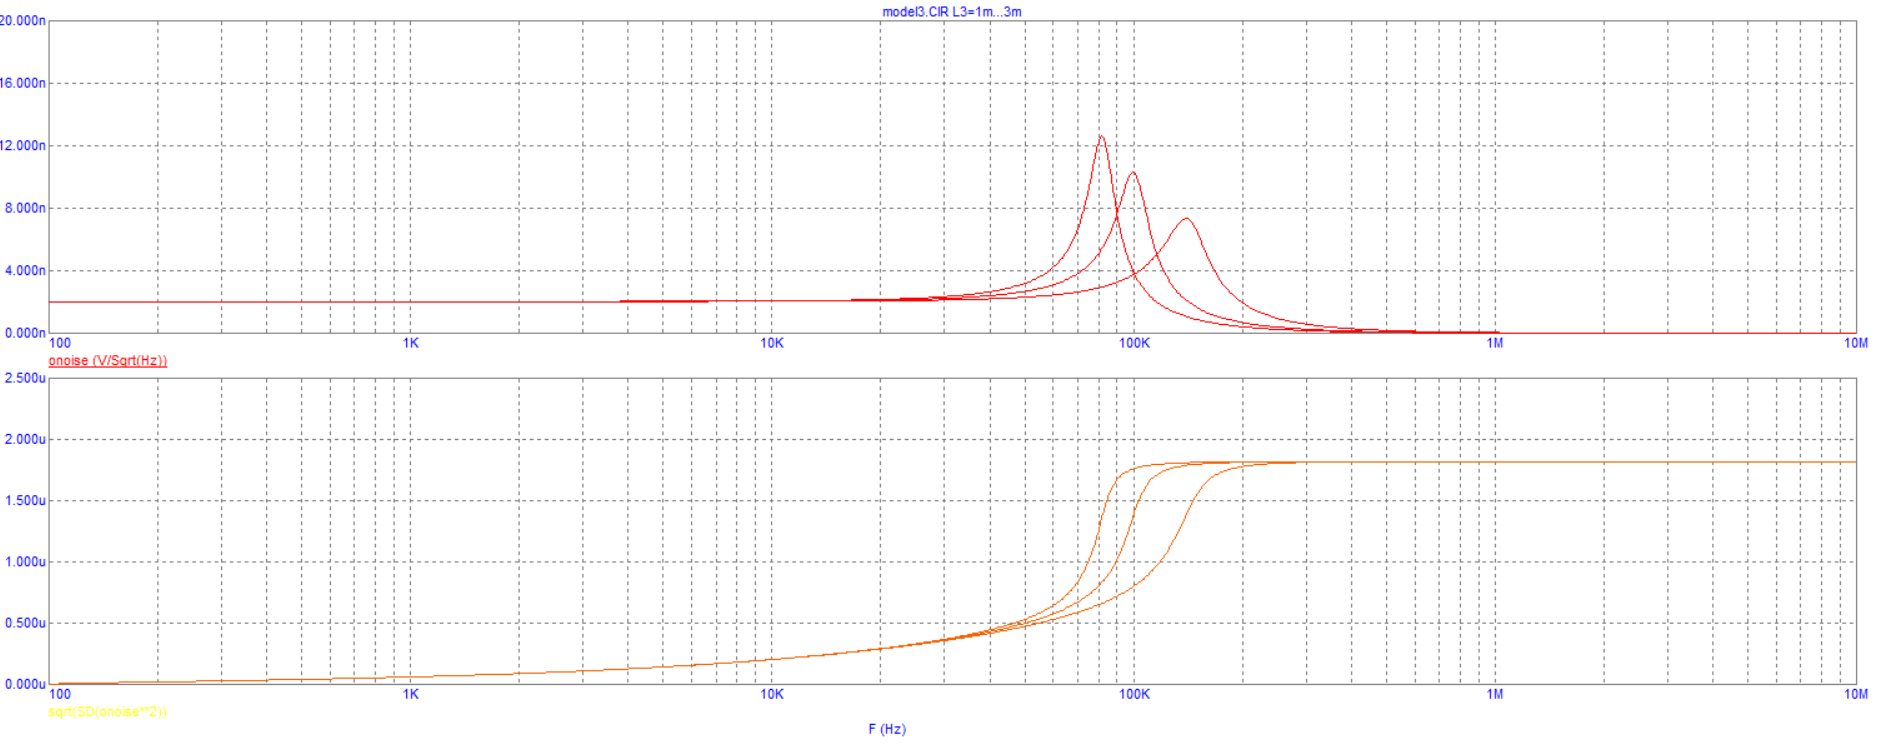
\includegraphics[scale=0.3]{images/mod3_3_2_3.png}
    \caption{Варьирование L3 = [1m, 3m |1m]}
    \label{fig:m3323}
\end{figure}

\begin{center}
\begin{tabular}{|c|c|c|c|}
\hline
    L3 & 1m & 2m & 3m\\ \hline
    $n_3(f_0)$ & 7.4n & 10.2n & 12.6n\\ \hline
    $n_3(f_0/10)$ & 2.1n & 2.1n & 2.1n \\ \hline
    $\sigma$ & 1.8$\mu$ & 1.8$\mu$ & 1.8$\mu$ \\ \hline
\end{tabular}
\end{center}

\end{enumerate}

\subsection*{LC-фильтр верхних частот}

\newpage

\begin{enumerate}

\item

.

\begin{figure}[h!]
    \centering
    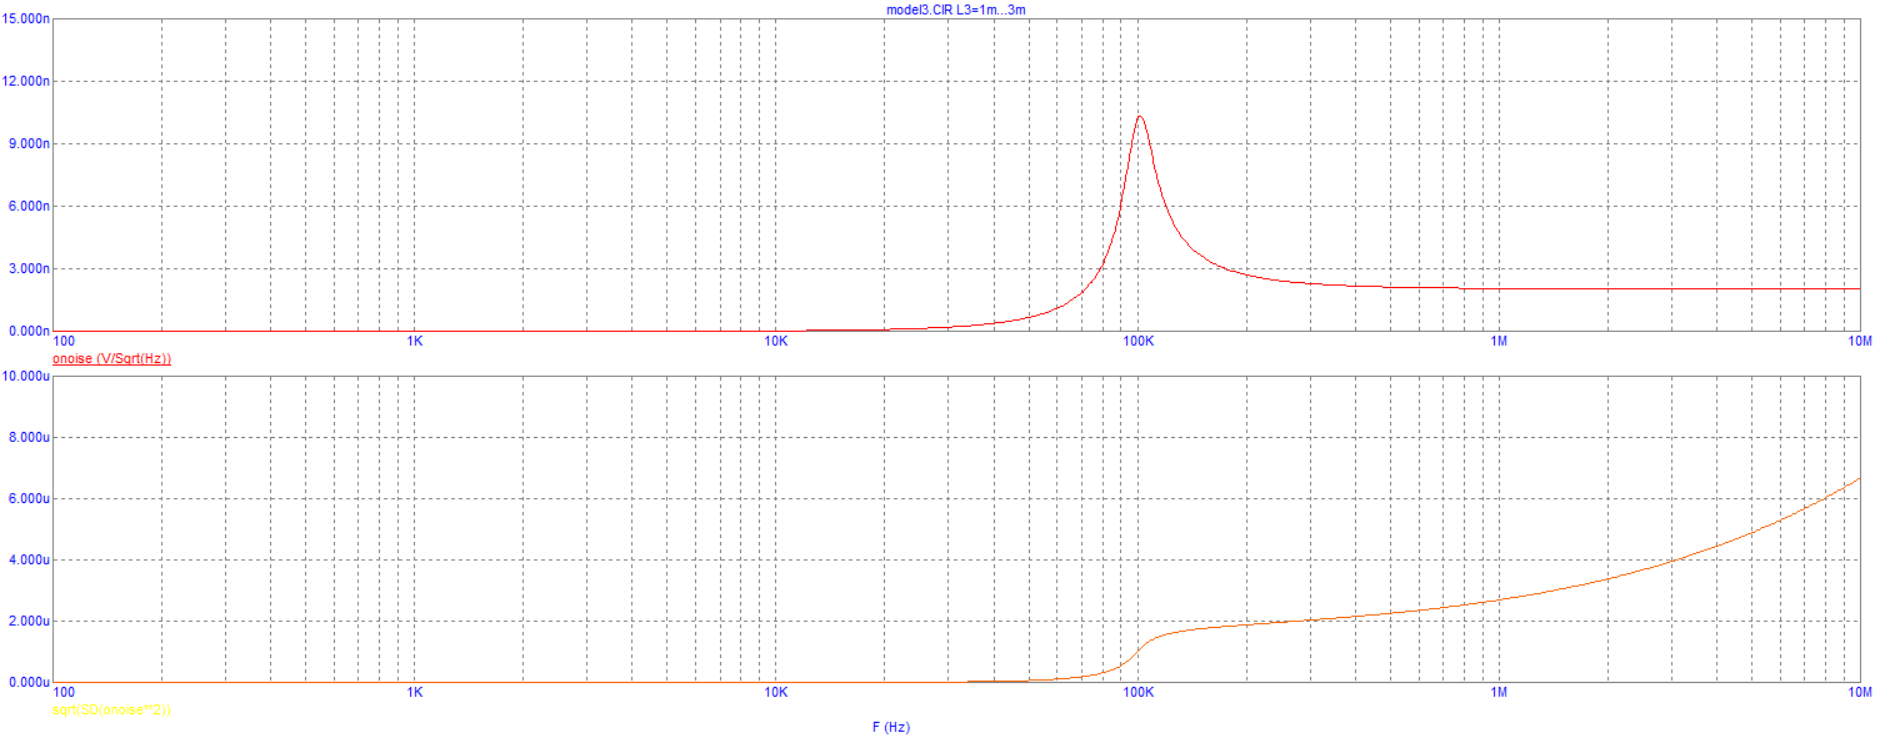
\includegraphics[scale=0.3]{images/mod3_4_1.png}
    \caption{$n_4(f_0) = 10.3n, n_4(10 f_0) = 2.0n, \sigma = 2.7\mu$}
    \label{fig:m341}
\end{figure}

Разумеется значение $n_4(10 f_0)$ будет совпадать с шумовым напряжением резистора, поскольку при высоких частотах фильтр себя не проявляет(конденсатор - провод, катушка - обрыв) и весь шум идет от резистора на узел n3.

\begin{figure}[h!]
    \centering
    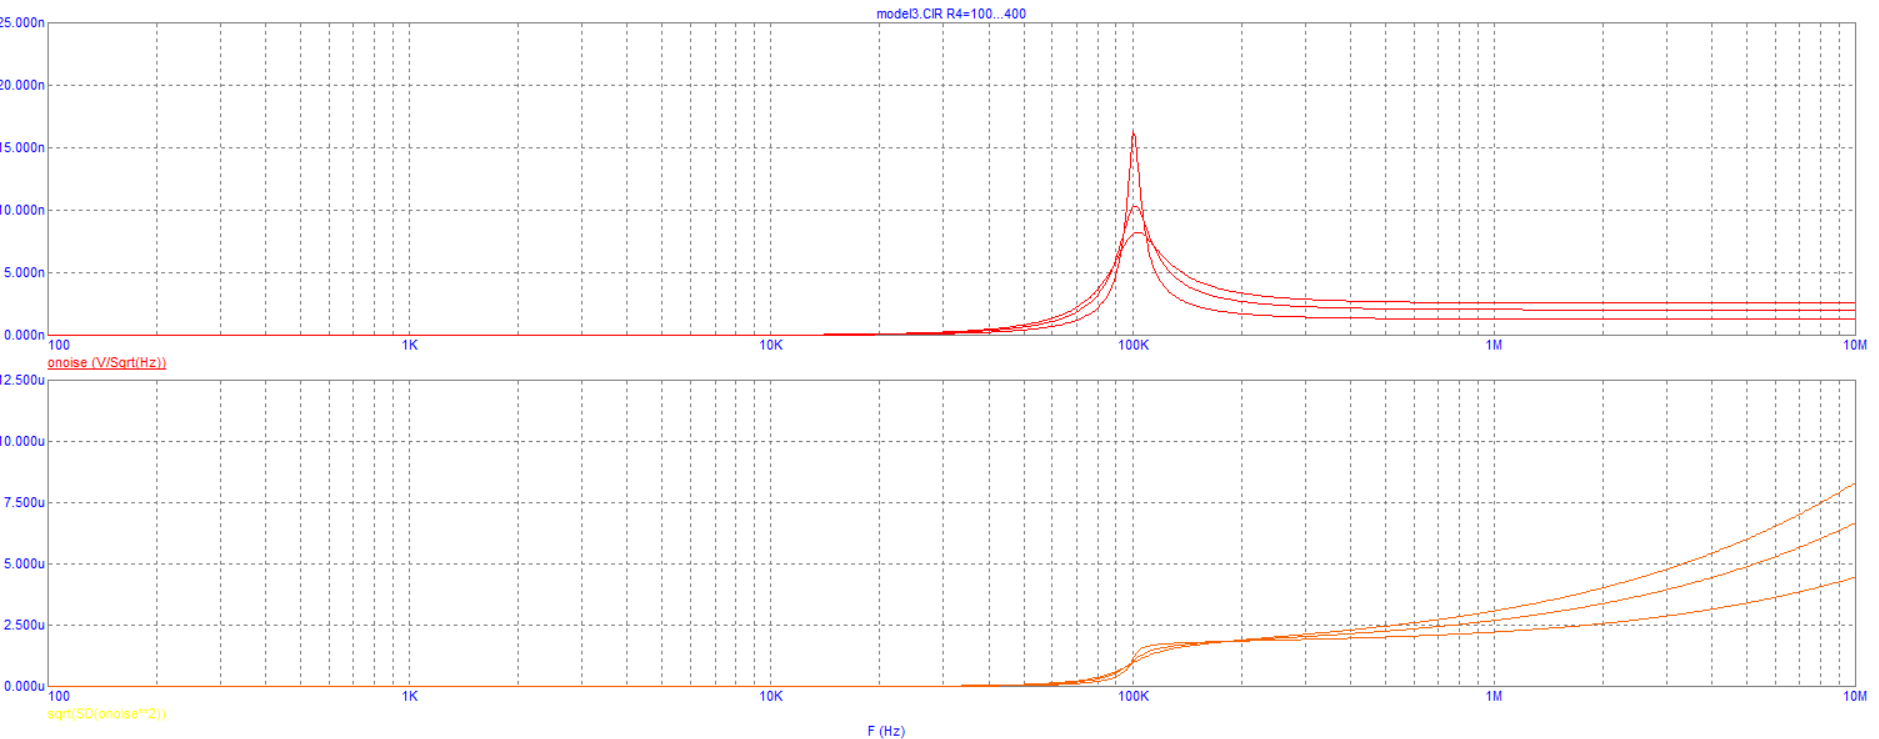
\includegraphics[scale=0.3]{images/mod3_4_2_1.png}
    \caption{Варьирование R4 = [100,400|150]}
    \label{fig:m3421}
\end{figure}

\begin{center}
\begin{tabular}{|c|c|c|c|}
\hline
    R3 & 400 & 250 & 100\\ \hline
    $n_4(f_0)$ & 8.2n & 10.2n & 15.9n\\ \hline
    $n_4(10 f_0)$ & 1.1n & 2n & 2.6n\\ \hline
    $\sigma(10 f_0)$ & 3.0$\mu$ & 2.7$\mu$ & 2.2 $\mu$ \\ \hline
\end{tabular}
\end{center}

\newpage

\begin{figure}[h!]
    \centering
    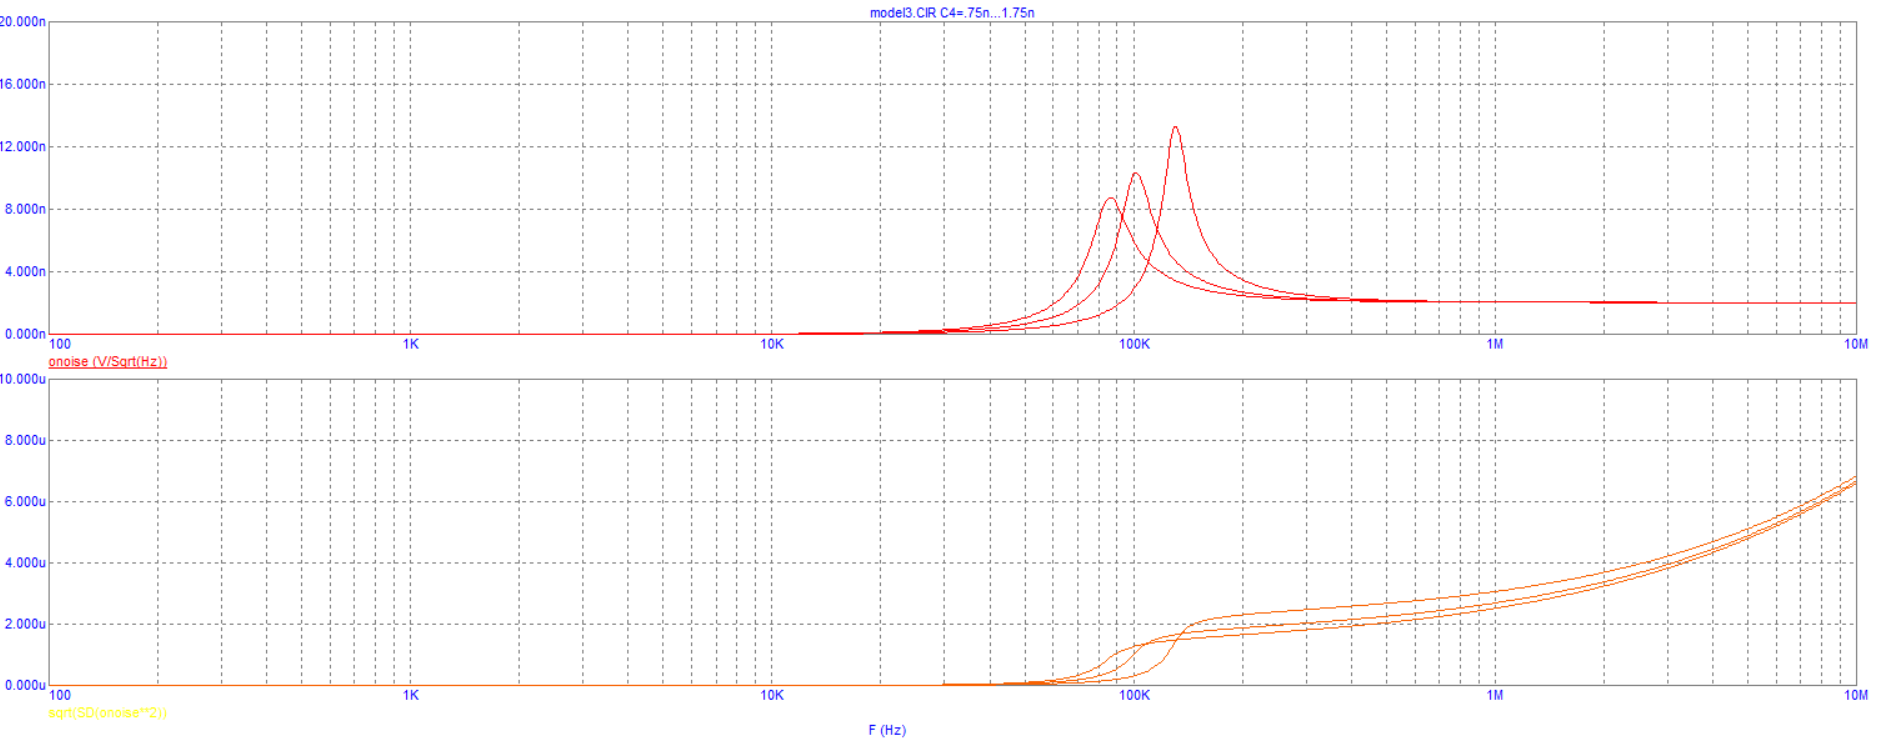
\includegraphics[scale=0.3]{images/mod3_4_2_2.png}
    \caption{Варьирование C4 = [0.75n, 1.75n |0.5n]}
    \label{fig:m3422}
\end{figure}

\begin{center}
\begin{tabular}{|c|c|c|c|}
\hline
    C4 & 0.75n & 1.25n & 1.75n\\ \hline
    $n_4(f_0)$ & 13.4n & 10.2n & 8.6n\\ \hline
    $n_4(10 f_0)$ & 1.9n & 1.9n & 1.9n \\ \hline
    $\sigma(10 f_0)$ & 3.1$\mu$ & 2.7$\mu$ & 2.5$\mu$\\ \hline
\end{tabular}
\end{center}

\begin{figure}[h!]
    \centering
    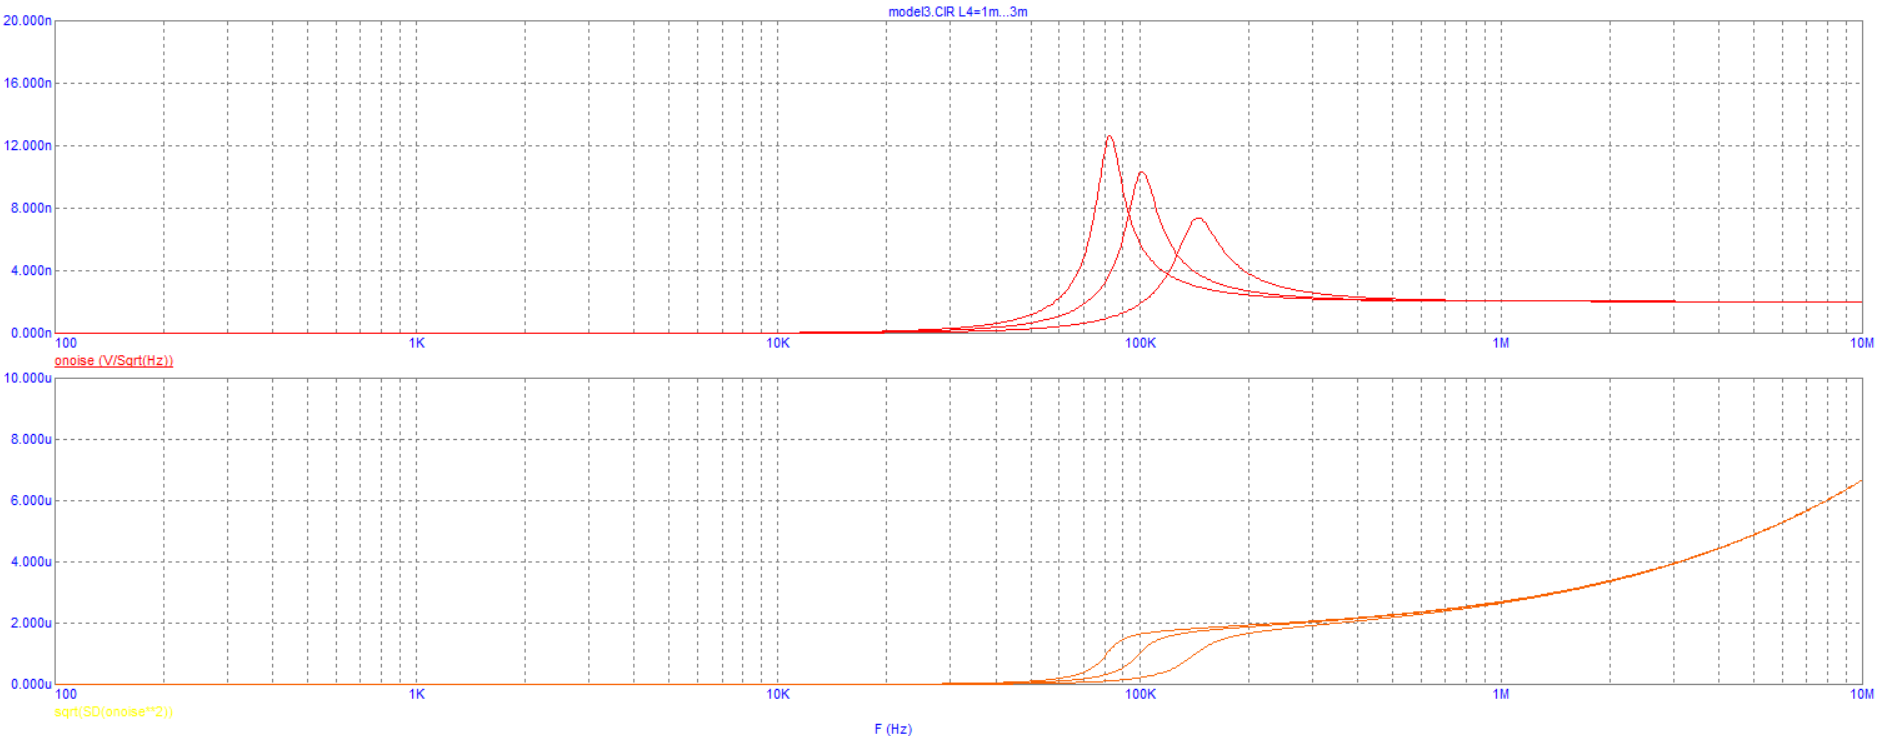
\includegraphics[scale=0.3]{images/mod3_4_2_3.png}
    \caption{Варьирование L4 = [1m, 3m |1m]}
    \label{fig:m3423}
\end{figure}

\begin{center}
\begin{tabular}{|c|c|c|c|}
\hline
    L3 & 1m & 2m & 3m\\ \hline
    $n_4(f_0)$ & 7.4n & 10.4n & 12.6n\\ \hline
    $n_4(10 f_0)$ & 2.0n & 2.0n & 2.0n \\ \hline
    $\sigma(10 f_0)$ & 2.6$\mu$ & 2.6$\mu$ & 2.6$\mu$ \\ \hline
\end{tabular}
\end{center}

\end{enumerate}

\section{\textbf{model 4 (Шумящие фильтры)}}

\subsection*{Полосовой LC-фильтр}

\begin{enumerate}

\item

Параметры первого фильтра: $f_0 = 100 kHz, \rho = 1260, Q = 3$

\begin{figure}[h!]
    \centering
    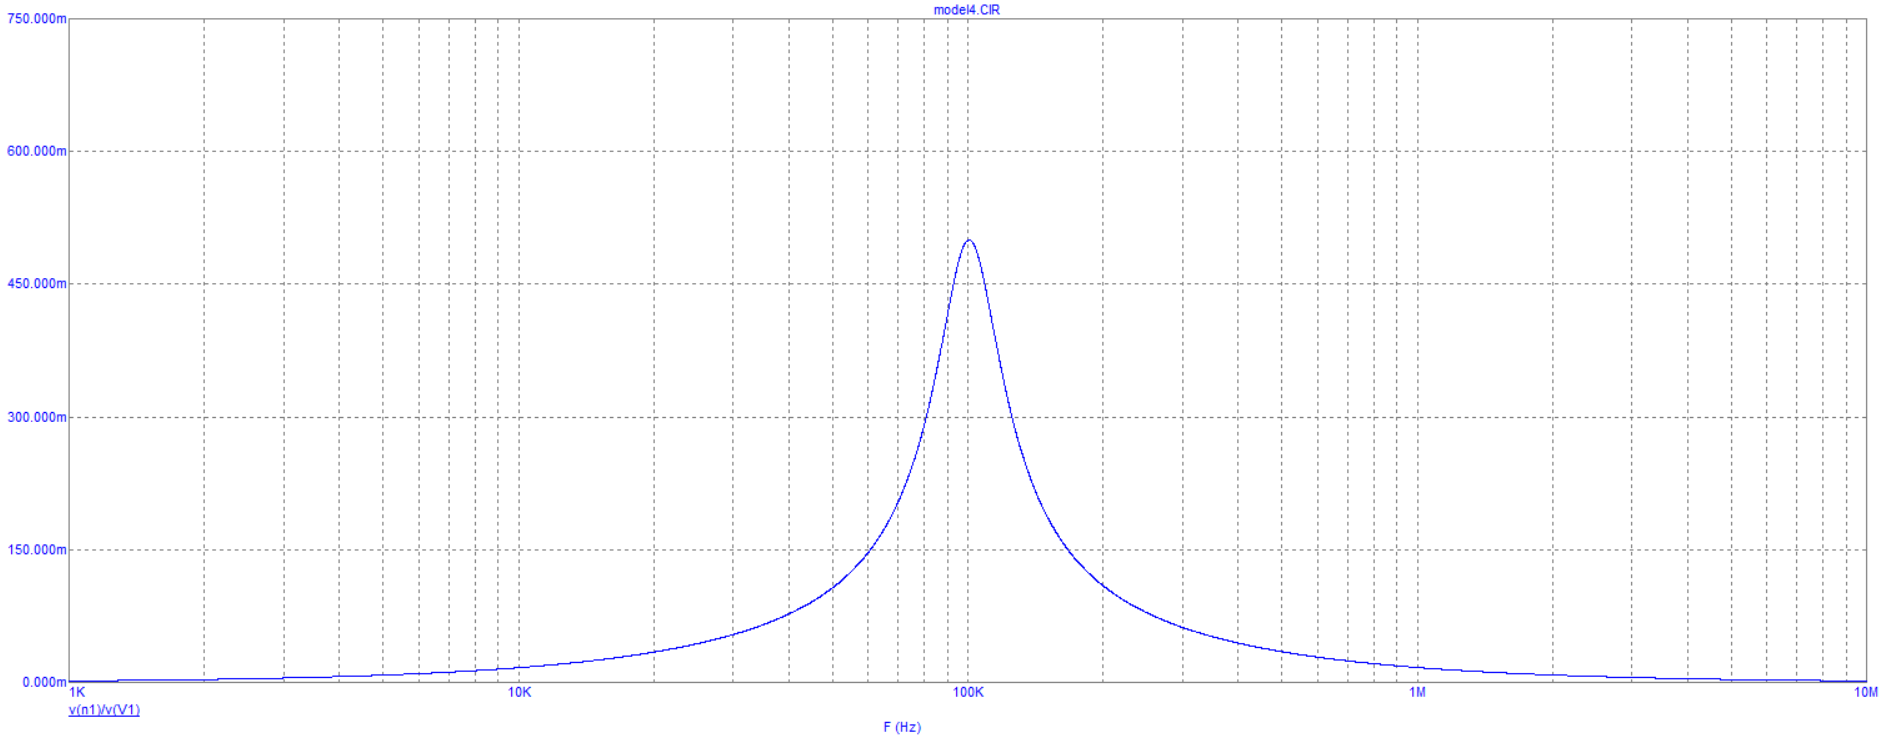
\includegraphics[scale=0.3]{images/mod4_1_1.png}
    \caption{$f_0 = 100K, \Delta f = 32K, K = 0.5$, с теорией соотносится}
    \label{fig:m411}
\end{figure}

\newpage

\item

.

\begin{figure}[h!]
    \centering
    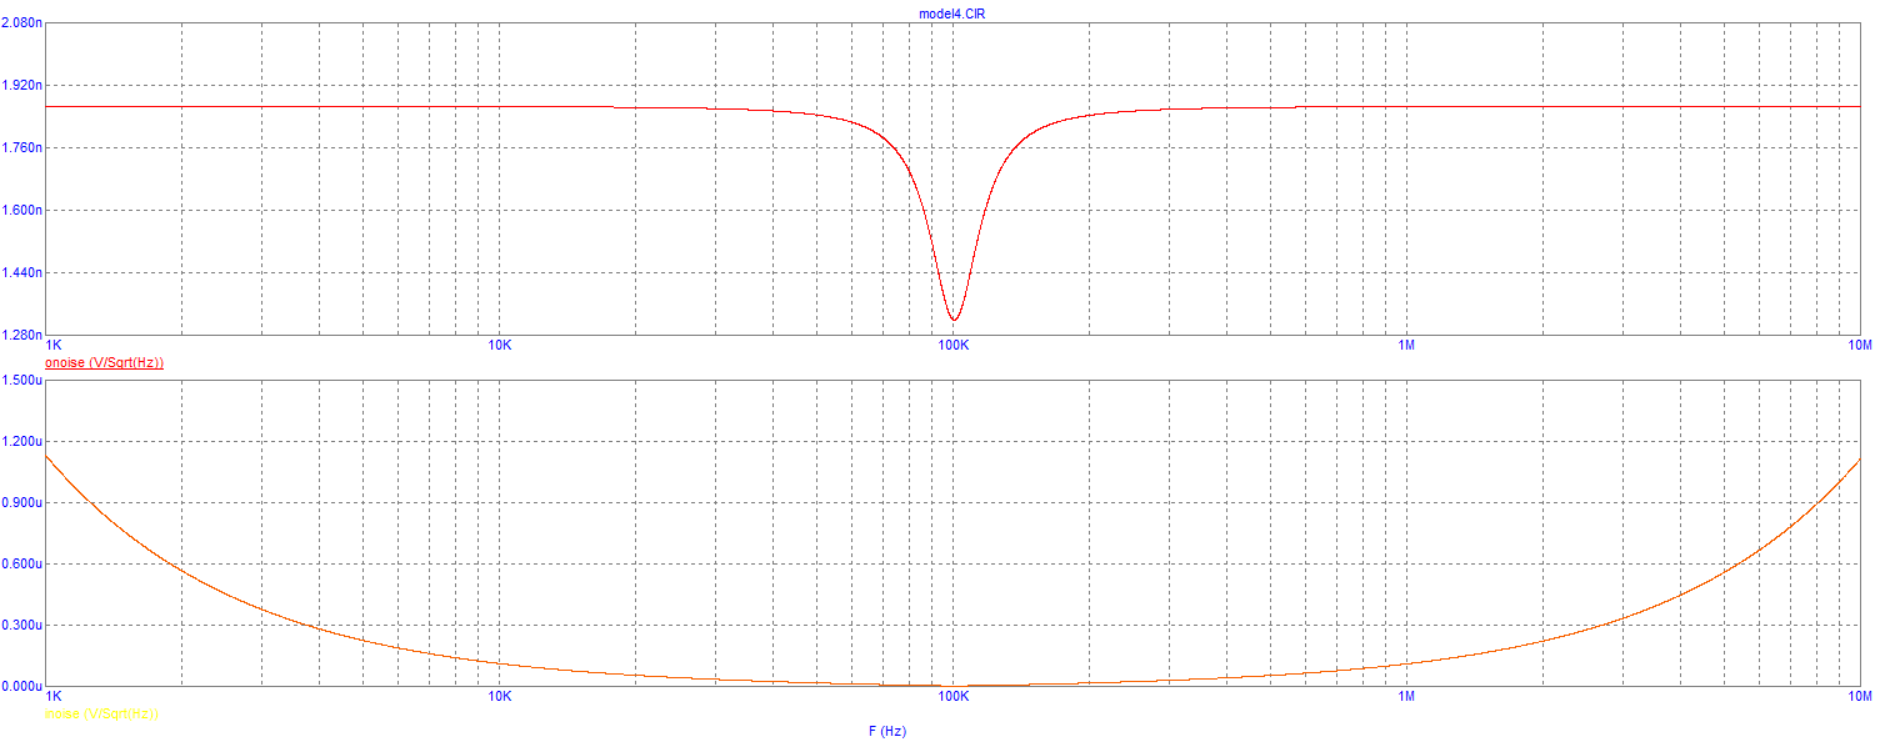
\includegraphics[scale=0.3]{images/mod4_1_2_1.png}
    \caption{$n(f_0) = 1.32n, n(f_0/10) = 1.89n, \sigma = 1.82\mu$, оба резистора шумящие}
    \label{fig:m4121}
\end{figure}

На частоте резонанса сопротивление последовательной LC-цепи становится нулевым. Тогда шум на выходе определяется параллельным соединением двух резисторов R. Вдали от резонанса высокий импеданс LC-цепи изолирует второй резистор от первого. Шум на выходе при этом увеличивается до шума e2 одного резистора R. Коэффициент же передачи максимален на резонансной частоте и быстро падает при уходе от нее. Поэтому коэффициент шума минимален в точке резонанса, оказываясь равным здесь коэффициенту шума делителя напряжения, и быстро растет при удалении от резонанса.

\newpage

.

\begin{figure}[h!]
    \centering
    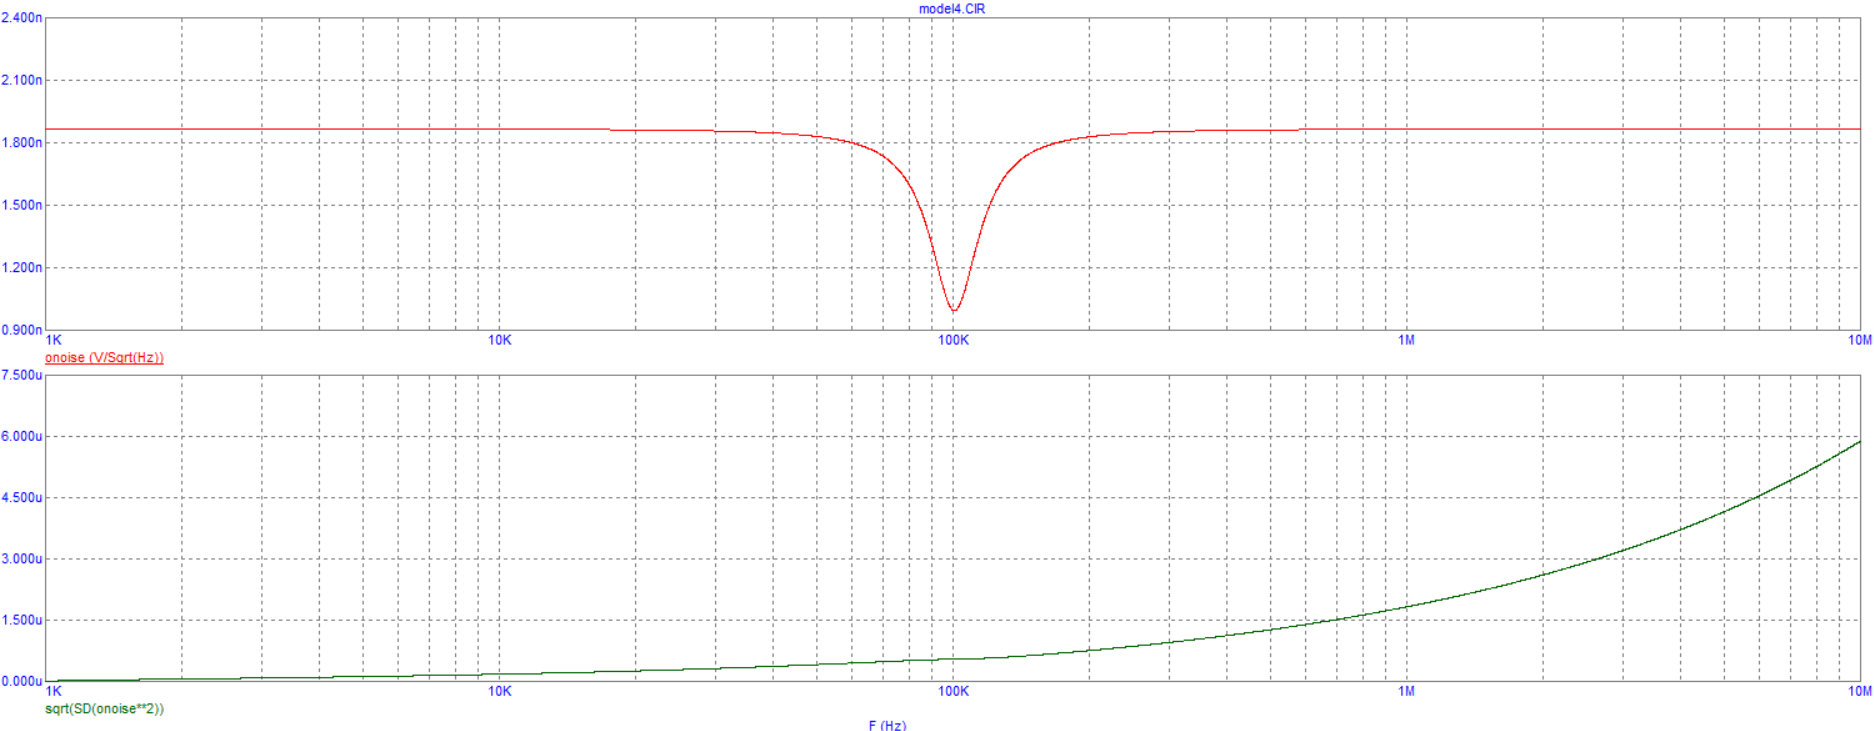
\includegraphics[scale=0.3]{images/mod4_1_2_2.png}
    \caption{$n(f_0) = 1.01n, n(f_0/10) = 1.86n, \sigma = 5.9 \mu$, $R_{s1}$ - не шумящий}
    \label{fig:m4122}
\end{figure}

.

\begin{figure}[h!]
    \centering
    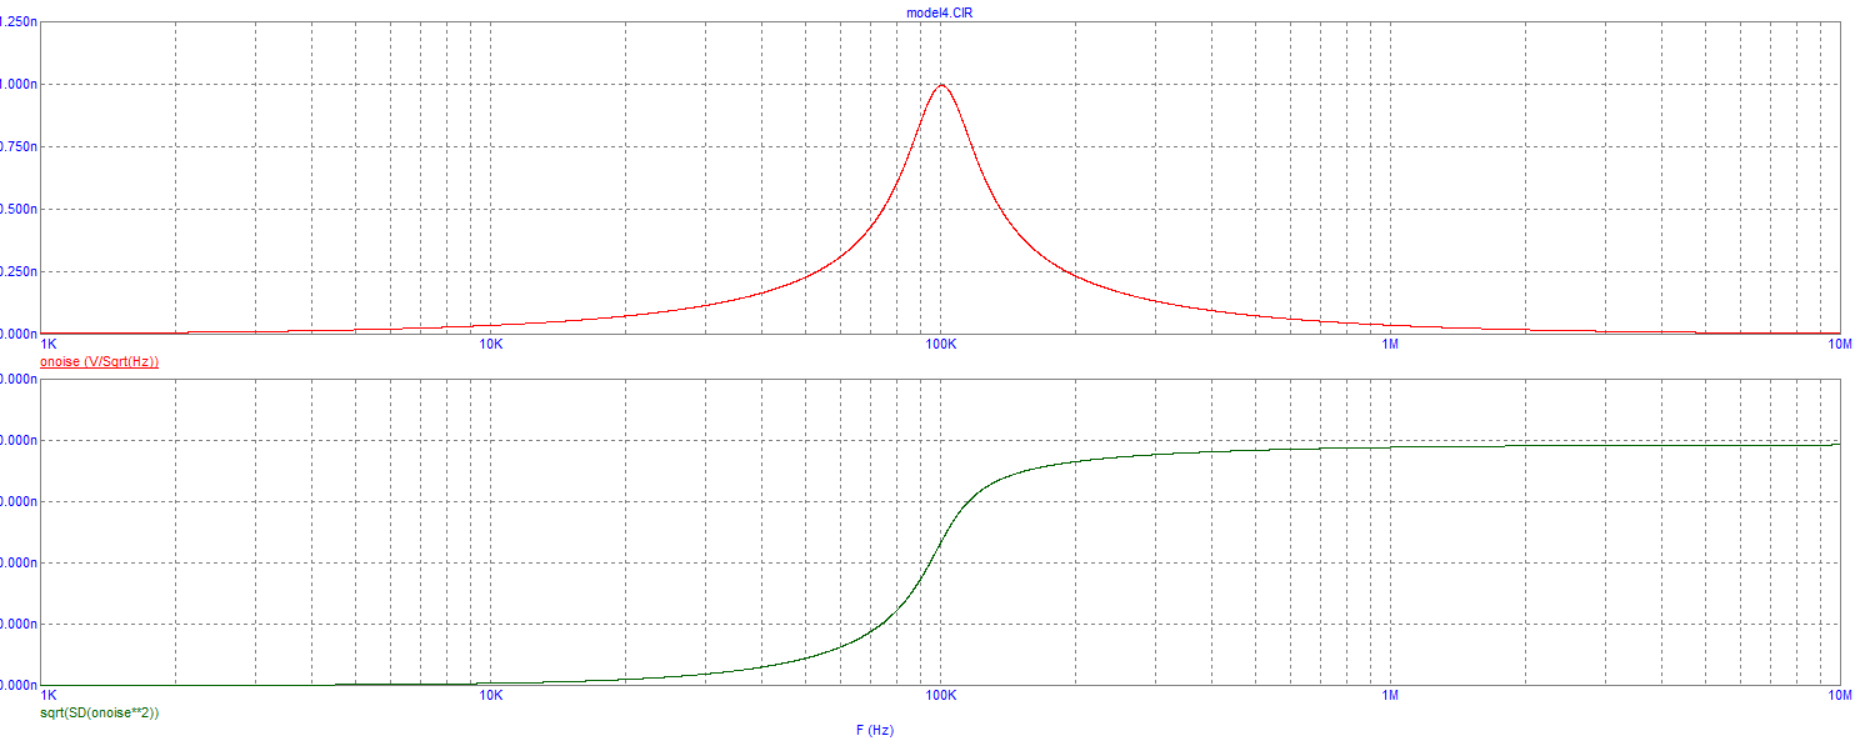
\includegraphics[scale=0.3]{images/mod4_1_2_3.png}
    \caption{$n(f_0) = 1.01n, n(f_0/10) = 30p, \sigma = 240n$, $R_1$ - не шумящий}
    \label{fig:m4122}
\end{figure}

Для частоты $f_0 / 10$ закон очевидно выполнен. Для частоты $f_0$, учитывая формулу параллельного соединения резисторов, получим требуемое соответствие.


\item
.

Формула коэффициента шума $K = 20 lg \left( \frac{e_n(f)}{\sqrt{4 k T R}} \right)$

\begin{figure}[h!]
    \centering
    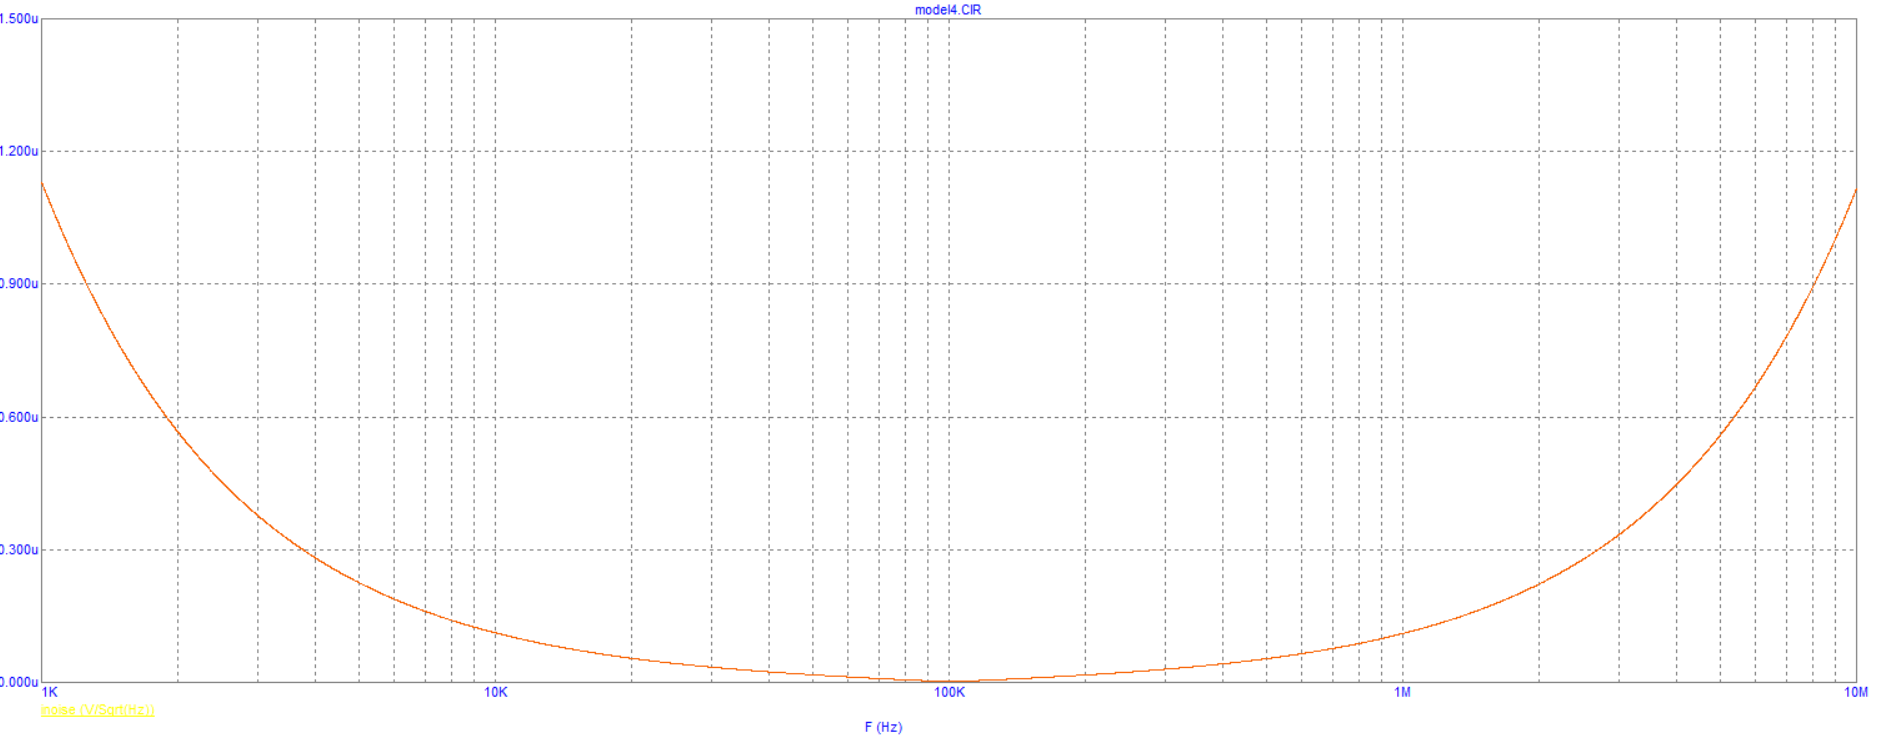
\includegraphics[scale=0.3]{images/mod4_1_3.png}
    \caption{$e(f_0) = 2.6n, e(f_0/10) = 110.1n => K_n(f_0 / 10) \approx 36, K_n(f_0) \approx 3$}
    \label{fig:m413}
\end{figure}

\end{enumerate}

\end{problem}
\end{document}